\documentclass[
  digital, %% Replace with `printed` to enable the default options for the printed version
  oneside,
  notable, %% `table` causes the coloring of tables. Replace with `notable` to restore plain tables.
  nolof,     %% `lof` prints the List of Figures. Replace with `nolof` to hide the List of Figures.
  nolot     %% `lot` rints the List of Tables. Replace with `nolot` to hide the List of Tables.
  %% More options are listed in the user guide at
  %% <http://mirrors.ctan.org/macros/latex/contrib/fithesis/guide/mu/fi.pdf>.
]{fithesis3}
\usepackage[utf8]{inputenc}
\usepackage{textcomp}
\usepackage{color}
\usepackage[hyphens]{url}
\usepackage{multirow}
\usepackage{seqsplit}


%% The following section sets up the locales used in the thesis.
%\usepackage[resetfonts]{cmap} %% We need to load the T2A font encoding
%\usepackage[T1,T2A]{fontenc}  %% to use the Cyrillic fonts with Russian texts.



\thesissetup{
    date          = 2017/05/22,
    university    = mu,
    faculty       = fi,
    type          = mgr,
    author        = {Josef Pavelec},
    gender        = m,
    advisor       = {RNDr. Andriy Stetsko, PhD.},
    title         = {Optimization of JVM settings for application performance},
    keywords      = {JVM settings, Optimization},
%%    TeXkeywords   = {keyword1, keyword2, \ldots},
}
\thesislong{abstract}{
    Will be written in the end.
}
\thesislong{thanks}{
    Will be written in the end.
}



%%% ======================================================= %%%

\begin{document}
\chapter{Introduction}
    Will be written in the end.

%%% ======================================================= %%%
\chapter{Java Virtual Machine}

Java Virtual Machine (JVM) is an abstract computing machine. JVM can not process any program written in Java language (stored in \texttt{java} source file) but it executes only the program called \textit{bytecode} which is stored in a \texttt{class} file. A Java \texttt{class} file is produced from \texttt{java} source file by Java compiler (\texttt{javac program.java} command). JVM, like a real computing machine, has its own instruction set for processing \textit{bytecode}. For running compiled Java program, it's necessary to have only an implementation of JVM for a given platform. Described approach offers the ability for applications to be developed in a platform-independent manner, and it can be shortened by Sun Microsystems slogan: "\textit{Write once, run anywhere}". \cite{spec}

In the context of the JVM it should distinguish three terms:
\begin{itemize}
	\item "\textbf{specification} is a document that formally describes what is required of a JVM implementation.
	\item \textbf{implementation} is a computer program that meets the requirements of the JVM specification.
	\item \textbf{instance} is an implementation running in a process that executes a computer program compiled into Java bytecode." \cite{brief}
\end{itemize}

For the correct implementation of Java Virtual Machine you only need to be able to read \texttt{class} file and perform the specified operations. The Java Virtual Machine specification doesn't contains any requirements or constraints for implementation of JVM. For this reason, the memory layout of run-time data areas, the garbage-collection algorithm used, any internal optimization of the JVM instruction (e.g. translating them into native code) and other matters connected with implementation of JVM are left to the implementor. Consequently, the JVM specification doesn't describe the possible ways how to adjust a JVM behaviour to achieve a better performance of a running application. \cite{spec}

There are many implementations of JVM\footnote{An extensive list of JVM implementation is accessible on \url{https://en.wikipedia.org/wiki/List_of_Java_virtual_machines}}. This chapter of the thesis deals with the Java HotSpot Virtual Machine respective to Java Development Kit 8 (JDK 8) which is the primary reference JVM implementation. This version is the latest because JDK 9 release is scheduled for July 2017\footnote{\url{https://blogs.oracle.com/java/proposed-schedule-change-for-java-9}}.

\section{Java HotSpot VM}
The Java 8 HotSpot Virtual Machine implementation is maintained by Oracle corporation. It implements JVM 8 specification and seeks to achieve best results for executing \textit{bytecode} in areas such as automatic memory management or compilation to native code.

Since the first version of JVM was interpreted, the statement "\textit{Java is slow}" has persisted notwithstanding it's not true in these days. More information regarding this topic will be provided in next sections.

\section{Compilation}

As mentioned earlier, the main purpose of JVM is executing \textit{bytecode} on a specific platform which means translating \textit{bytecode} to native code of CPU. Since interpreting of \textit{bytecode} had appeared inefficient, an approach called \textit{Just-In-Time} compilation (JIT) was introduced in Java 1.2 \cite{javavsc}. A JVM implementation with JIT compiler translates a program into native code on the fly. Native code is cached and reused without recompiled. The extent of native code optimization is limited in this case because translation should be fast.

Java HotSpot VM is appropriately named after approach it takes toward compiling the code. A small part of the code is executed frequently in common programs. Frequent code sections represent approximately 20 \%\footnote{\url{http://artiomg.blogspot.cz/2011/10/just-in-time-compiler-jit-in-hotspot.html}} which are in accordance with the Pareto principle. These sections are called \textit{hot spots}. The more the section of code is executed, the hotter section is said to be. The faster will be \textit{hot spots} executed, the higher performance of an application will be. \cite{scott}

Oracle's HotSpot VM combines interpretation and translation. First, it interprets all code and concurrently collects information how often code is executed and additional data. After that JVM uses collected information for compilation with a high level of optimization. The more information about code JVM has, the more level of optimization it can achieve but for the price of the slow interpretation in the beginning. Actually, depending on the aggressiveness and level of optimization there are two different compilers in HotSpot JVM -- \textbf{client} and \textbf{server} (see sections \ref{clientcomp} and \ref{servercomp}).

The choice of which compiler to use is often the only one decision that is done during the compiler tuning. Even, choosing of compiler must be considered before JVM is installed because different JVM binaries contain different compilers. \cite{scott}

%Another important role of any JVM implementations is automatic memory management known as \textbf{Garbage collections (GC)} (see section \ref{memory}). There are four different algorithms (called as Garbage Collectors) that provide this task in a HotSpot:
%\begin{itemize}
%	\item \textbf{serial collector}
%	\item \textbf{parallel (throughput) collector}
%	\item \textbf{concurrent (CMS) collector}
%	\item \textbf{G1 collector}
%\end{itemize}
%Every of garbage collectors has quite a different performance characteristics and is suitable for a different category of an application and environment. \cite{scott}

\subsection{Client compiler}\label{clientcomp}
The HotSpot VM's client compiler is designed for faster application startup, quick compilation and smaller memory footprint. This type of compiler is typically suitable for GUI application because there is a responsiveness without jitter desired. \cite{hunt}

The name \textit{client} compiler comes from the command-line argument \texttt{-client} used to select the compiler. When 64-bit version of the JDK is used, this option is ignored and \textit{server} compiler (see section \ref{servercomp}) will be used. Sometimes client compiler is called \textit{compiler 1} or shortly \textit{C1}\footnote{The short notation is used in list of advanced options. See section \ref{secoptions}}. \cite{scott} \cite{java}
\subsection{Server compiler}\label{servercomp}
The second HotSpot VM's compiler targets high throughput and peak performance. The server compiler uses the most powerful optimizations it can. The disadvantage of this behaviour is a fact, that time for getting an essential information for top optimization can be long. Concurrently, the overall memory footprint of server compiler is larger due to more data to handle. Native code produced by server compiler will be definitely more effective. Therefore advantages of high optimization of code depend on a run time of an application and the server compiler is suitable for long running applications. \cite{hunt}

The \texttt{-server} option serves for use the server compiler. The server compiler is also marked as \textit{compiler 2} or \textit{C2}.

A technique called \textit{tiered compilation} combines a client compiler fast startup and a server compiler high optimization. With the tiered compilation, the code is first compiled by the client compiler, as it becomes hot, it is recompiled by the server compiler. The tiered compilation is available only for server compiler\footnote{If command \texttt{java -client -XX:+TieredCompilation}\textit{ programName} is used, \texttt{-XX:+TieredCompilation} option is quietly turned off. \cite{scott}}. The tiered compilation was introduced in the JDK 7 and it becomes as default in the JDK 8. \cite{scott}
\section{Memory management}\label{memory}
The Java SE platform provides an automatic memory management. The JVM specification prescribes that any JVM implementation must ensure reclaiming unused memory -- unreachable objects also called \textit{garbage} or dead objects. A process of reclaiming unreachable objects is known as \textit{garbage collection} (GC). A developer does not care about complexity of memory allocation and \textit{garbage collection}. \cite{gctuning}

\begin{figure}[h]
	\centering
	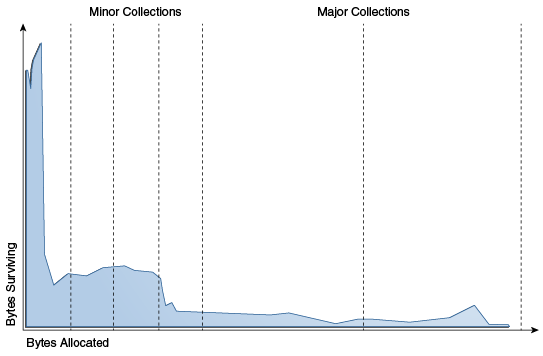
\includegraphics[width=10cm]{fig/survive.png}
	\caption{Typical distribution for lifetimes of objects. A majority of objects "die young". Taken from \cite{gctuning}.}
	\label{survive}
\end{figure}

The \textit{weak generational hypothesis} is generally true for Java applications which means: \cite{hunt}
\begin{itemize}
	\item "Most allocated objects become unreachable quickly.
	\item Few references from older to younger objects exist."
\end{itemize}

Therefore the Java HotSpot VM splits the heap\footnote{Heap is a memory area that JVM uses for residing the Java objects.} into two areas (also called spaces), which are referred to as generations: \cite{hunt}
\begin{itemize}
	\item \textbf{The young generation} -- the vast majority of new objects are allocated in this area. Most objects become into \textit{garbage} quickly and a small part of it survives a young generation collection -- \textit{minor} garbage collection. Reclaiming objects from this area is usually efficient because they occupy relatively a small space and mostly are dead. 
	\item \textbf{The old generation} -- long-live objects are moved (also called \textit{promoted} or \textit{tenured}) to the old generation. This area is also known as \textit{tenured} space. The old generation is usually larger than the young generation and it grows slowly. \textit{Garbage collection} in \textit{tenured} space -- \textit{major} garbage collection is less frequent, but it can be quite lengthy.
\end{itemize}

%TODO zkus vytisknout a podivat se, jak to bude vypadat
\begin{figure}[h]
	\centering
	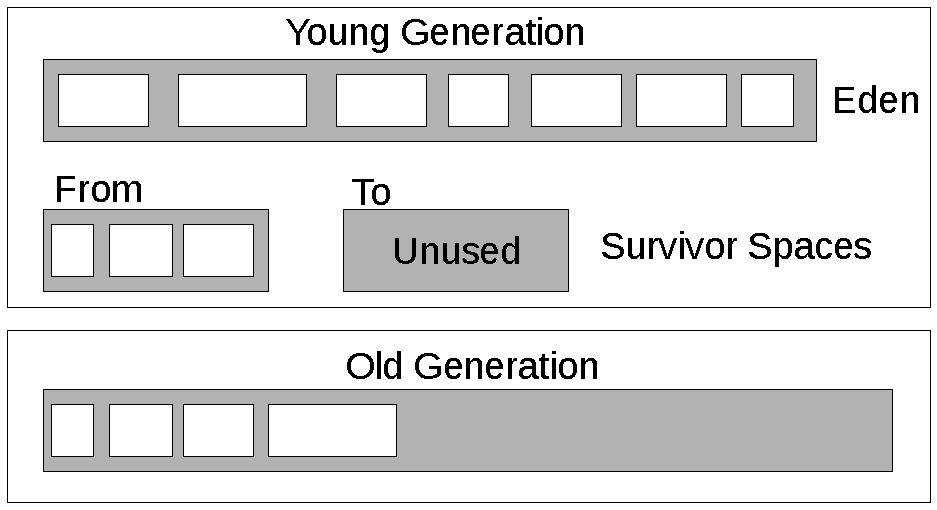
\includegraphics[width=7cm]{fig/heap.pdf}
	\caption{A Java HotSpot VM heap division. Adjusted from \cite{hunt}.}
	\label{heap}
\end{figure}

There is a more detailed heap division of JVM in the figure \ref{heap}. The young generation contains \textit{Eden} space and two \textit{Survivor} spaces. Almost all new objects are allocated in \textit{Eden} space (large objects can be allocated directly in the old generation) and if an object is live after at least one \textit{minor} garbage collection it moves to one of \textit{Survivor} space. The object has to be reachable after several \textit{minor} garbage collection to \textit{promoted} to the old generation. One of \textit{Survivor} space remains unused. A \textit{minor} garbage collection process is depicted in figure \ref{minor}.

%TODO zkus vytisknout a podivat se, jak to bude vypadat
\begin{figure}[h]
	\centering
	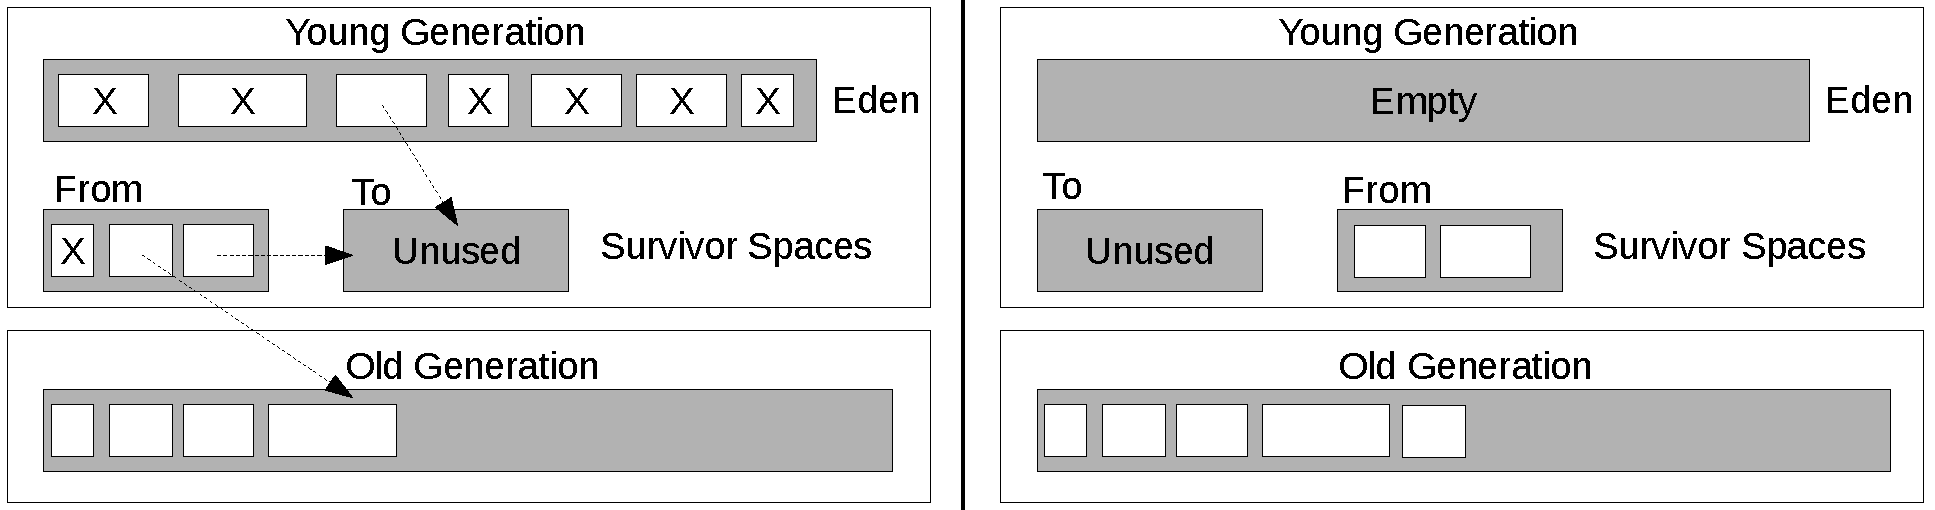
\includegraphics[width=13cm]{fig/minor.pdf}
	\caption{\textit{Minor} garbage collection. Objects with a cross on left side are unreachable. Adjusted from \cite{hunt}.}
	\label{minor}
\end{figure}

Compared to previous Java version, there is a one essential change in a Java 8 memory management. There is not \textit{Permanent} space anymore. Instead of this memory area we can find a \textit{Metaspace} in a current JVM. Both areas serve for storing class and method objects. As seen in the figure \ref{metaspace}, \textit{Permanent} generation is in heap while \textit{Metaspace} is not. It is part of native memory (process memory) which is only limited by the host operating system. \cite{metaspace}

\begin{figure}[h]
	\centering
	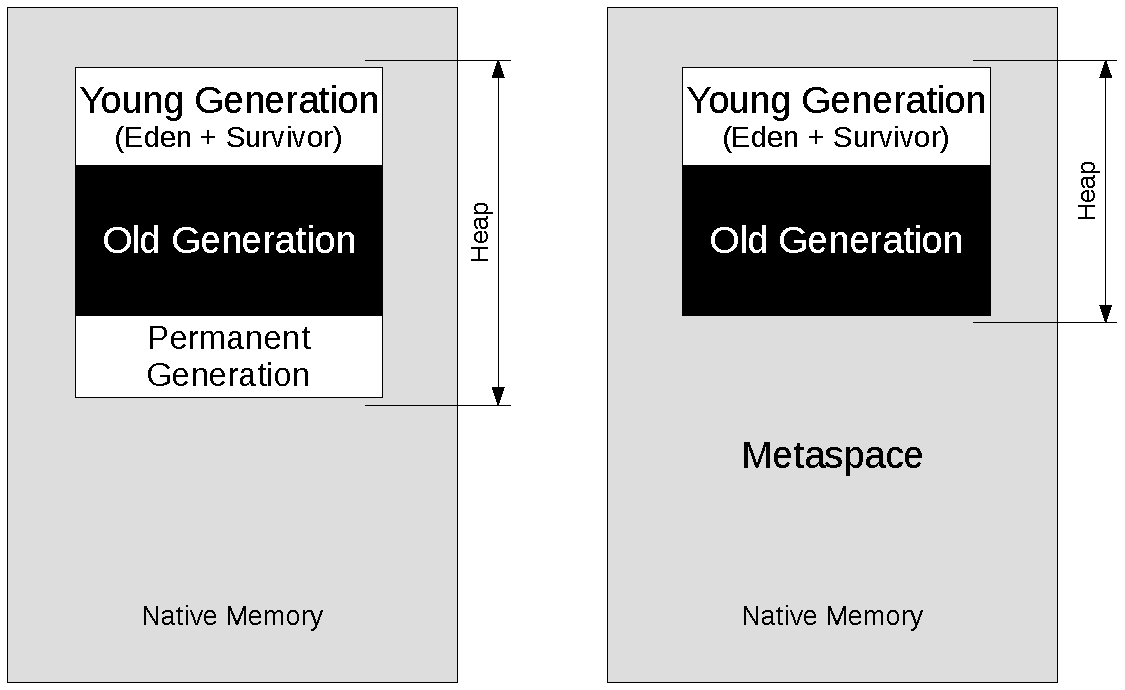
\includegraphics[width=10cm]{fig/metaspace.pdf}
	\caption{A permanent space (generation) has replaced \textit{Metaspace}. Adjusted from \cite{metaspace}.}
	\label{metaspace}
\end{figure}


% http://karunsubramanian.com/websphere/one-important-change-in-memory-management-in-java-8/ a metaspace
% - velke objekty jdou rovnou do ... (dopln cast). Limit, kterym se nastavuje mez je pomoci -XXtlaSize and -XXlargeObjectLimit -- prozkoumat

\section{Garbage collectors}
	\subsection{Serial collector}
	\subsection{Parallel collector}
	\subsection{(CMS) collector}
	\subsection{G1 collector}

\section{Setting options}\label{secoptions}
There are many options how to adjust JVM behaviour. For example, we may enforce to use parallel collector or set maximum heap size. Options are divided into several categories:
\begin{itemize}
	\item "\textbf{Standard options} -- are guaranteed to be supported by all implementations of the Java Virtual Machine (JVM). They are used for common actions, such as checking the version of the JRE, setting the class path, enabling verbose output, and so on.
	\item \textbf{Non-standard options} -- are general purpose options that are specific to the Java HotSpot Virtual Machine, so they are not guaranteed to be supported by all JVM implementations, and are subject to change. These options start with \texttt{-X}.
	\item \textbf{Advanced options} -- are not recommended for casual use. These are developer options used for tuning specific areas of the Java HotSpot Virtual Machine operation that often have specific system requirements and may require privileged access to system configuration parameters. They are also not guaranteed to be supported by all JVM implementations, and are subject to change. Advanced options start with \texttt{-XX}." \cite{java}
\end{itemize}
For listing all standard options is used the command \texttt{java -?} and non-standard options \texttt{java -X}. A situation for listing advanced options becomes little complicated because we have to make a decision which supersets of advanced option we want to list. On the other hand, diagnostic options superset is not the point of interest in this thesis because these options not meant for VM tuning or for product mode. Similarly commercial features. Therefore, for listing advanced options which are relevant for this thesis command \texttt{java -XX:+PrintFlagsFinal -XX:+UnlockExperimentalVMOptions} was used. List of advanced options contains option name, type (e.g. bool, (u)intx, ccstr) and default value (see section \ref{secerg}) and category (e.g. product, experimental).

Generally, there are two types of advanced options: boolean options, and options that require a parameter. The boolean options use the syntax: \texttt{-XX:+OptionName} enables the option, and \texttt{-XX:-OptionName} disables the option. Options with parameter use syntax: \texttt{\seqsplit{-XX:OptionName=value}}, meaning to set the value of \texttt{OptionName} to \texttt{value}. \cite{scott}



\section{Java ergonomics}\label{secerg}
This term covers the process by which the JVM provides a platform-dependent default selections. It aims to reduce the number of user defined used options and mainly improve the performance of running application. In addition, behaviour-based tuning dynamically tunes the sizes of the heap to achieve a smaller memory footprint and to meet a specified behaviour of the application. Depending on the environment features where the JVM runs can be defined the \textit{Server-class} machine. A machine is considered the \textit{Server-class} when meets next requirements:
\begin{itemize}
	\item 2 or more physical processors
	\item 2 or more GB of physical memory
\end{itemize}
The table \ref{figerg} shows what a compiler will be used for given platform. If JVM runs on the \textit{Server-class} machine, it uses the \textit{server} compiler with the exception of 32-bit platforms running a version of the Windows operating system.

\begin{table}[]
	\centering
	\begin{tabular}{|l|l|l|l|}
		\hline
		\textbf{Platform} & \textbf{Operating System} & \textbf{Default} & \textbf{Server-Class} \\ \hline
		i586              & Linux                     & Client           & Server                           \\ \hline
		i586              & Windows                   & Client           & Client                           \\ \hline
		SPARC (64-bit)    & Solaris                   & Server           & Server                           \\ \hline
		AMD (64-bit)      & Linux                     & Server           & Server                           \\ \hline
		AMD (64-bit)      & Windows                   & Server           & Server                           \\ \hline
	\end{tabular}
	\caption{Determination the runtime compiler for different platforms. Taken from \cite{ergonomics}.}
	\label{figerg}
\end{table}

The Default values which are shown in the list produced by \texttt{java -XX:+PrintFlagsFinal -XX:+UnlockExperimentalVMOptions} command are based on the Java ergonomics. On the \textit{Server-class} machine, the following are selected by default:
\begin{itemize}
	\item Initial heap size of 1/64 of physical memory up to 1 GB
	\item Maximum heap size of 1/4 of physical memory up to 1 GB
	\item Parallel (throughput) garbage collector
\end{itemize}
Unless the initial and maximum heap sizes are specified on the command line, these values will be used. \cite{ergonomics}


\chapter{Methodology of choosing important options}
This chapter of thesis deals with a restriction of huge option set and determination options which have a considerable performance impact.

The set of options contains 815 options\footnote{The sum of 21 standard, 26 non-standard and 768 advanced (\texttt{java -XX:+PrintFlagsFinal -XX:+UnlockExperimentalVMOptions} command) options for Java HotSpot\texttrademark{} 64-Bit Server VM (build 25.111-b14, mixed mode).}. As described in the section \ref{secoptions}, there are several types of options in JVM\footnote{For example, advanced option set contains 383 boolean, 184 integer and 173 unsigned integer options. (Remaining option types are double, string (ccstr), etc.)}. If JVM options had only boolean type, JVM would have $2^{815}$ different settings. Testing all options is technically possible, but practically not.


The methodology of choosing important options is based on a study how the options influence the JVM behaviour. Firstly, a principles of execution \textit{bytecode} by JVM has been studied together with options which can adjust the execution. Based on the level influencing the JVM behaviour and availability a documentation it's possible to categorize JVM options into following groups:
\begin{itemize}
	\item \textbf{Big Impact}
	\item \textbf{Small Impact}
	\item \textbf{Not Relevant}
	\item \textbf{Not Documented}
\end{itemize}

Some options require a current use of another option -- typically garbage collectors have own specific options. For example, setting of \texttt{-XX:ConcGCThreads} option has the meaning only if the CMS or the G1 collector is used. Therefore, the first two groups of enumeration above are distributable into next two groups:
\begin{itemize}
	\item \textit{primitive} -- options from this set doesn't require enabling of "parent" option.
	\item \textit{complex} -- for use some option it's necessary to enable a certain "parent" option.
\end{itemize}
A big disadvantage is a fact, that JVM doesn't point out this incompatibility. Hence, when a command \texttt{\seqsplit{java\ -XX:+UseSerialGC\ -XX:ConcGCThreads=4}} \textit{programName} is launched, JVM executes \textit{programName} without taking \texttt{-XX:ConcGCThreads=4} option into account. There is least at least an option \texttt{-XX:IgnoreUnrecognizedVMOptions} (default \texttt{false}) in JVM and when it is disabled syntax and type errors are highlighted. For example, command \texttt{java -XX:+UseConcMarkSweepGC -XX:ConcGCThreads=-4 }\textit{programName} end with message: "Improperly specified VM option 'ConcGCThreads=-4'".

In picture \ref{classify} there is a way how all options of JVM was splitted.

\begin{figure}[h]
	\centering
	\includegraphics[width=10cm]{fig/classify.png}
	\caption{JVM options distribution into several categories with regard to performance impact and a documentation extent.}
	\label{classify}
\end{figure}

\section{Big impact}
These options were evaluated as most important for performance impact. The selection was based on the available Oracle's documentation (\cite{java}) and a literature dealing with the Java performance (\cite{scott}, \cite{hunt}).

The big impact options, according to the previously mentioned distribution, are composed by two subsets -- the \textit{primitive} (see a complete list of \textit{primitive} options in the appendix \ref{bigimpactprimitive}) and the \textit{complex} (see a complete list of \textit{complex} options in the appendix \ref{bigimpactcomplex}). These options are intended for further optimization (e.g. by using any tool described in section \ref{autoopt}).

Among the most important \textit{primitive} options are:
\begin{itemize}
	\item \texttt{-client | -server} -- choice of compiler. For more information about client compiler see section \ref{clientcomp} and server compiler see section \ref{servercomp}.
	\item \texttt{-d32 | -d64} -- when a 32-bit operating system is used, then it's required using a 32-bit version of the JVM. When a 64-bit operating system is used, then it's possible to choose 32-bit or 64-bit version of the JVM. The 32-bit version will be faster and have a smaller footprint\footnote{For the heaps up to 3 GB. \cite{scott}}. Because 32 bit memory references occupy smaller memory area and manipulating those references is less expensive. \cite{scott}
	\item \texttt{-Xmixed} -- interprets all bytecode except for hot methods, which are compiled to native code. \cite{java}
	\item \texttt{-Xcomp} -- forces compilation to native code on the first invocation of method. \cite{java}
	\item \texttt{-Xms<size>} -- sets initial Java heap size. \cite{java}
	\item \texttt{-Xmx<size>} -- sets maximum Java heap size \cite{java}. The JVM automatically sets the initial and maximum heap size (see section \ref{secerg}). Due to an application memory requirements, values initial and maximum heap size set by the JVM can be insufficient or uselessly great and their setting is a basic memory footprint tuning.
	\item \texttt{-XX:MaxGCPauseMillis} -- sets a target for the maximum GC pause time in milliseconds. This value is not guaranteed (it's soft goal) but JVM makes its best effort to achieve it.
\end{itemize}
Several \textit{complex} options with a big impact on the performance:
\begin{itemize}
	\item \texttt{-XX:TieredCompilation} -- is available only if \texttt{-server} option is enabled. It enables tiered compilation described in section \ref{servercomp}.
	\item \texttt{-XX:ParallelGCThreads} -- the setting this option makes sense only if another GC than serial GC is used. By default, one thread for every CPU runs for GC, up to eight CPUs. For machines with more than eight CPUs \texttt{-XX:ParallelGCThreads} option equals $8 + ((N - 8) * 5 / 8)$, where \textit{N} is a number of CPUs. When more JVM instances are running on the machine, it's a good idea to limit the total number of GC threads among all instances. GC threads are quite efficient and can consume 100 \% of single CPU.~\cite{scott}
	\item \texttt{-XX:ConcGCThreads} -- if \texttt{-XX:UseConcMarkSweepGC} or \texttt{-XX:Use\-G1GC} option is enabled the use of \texttt{-XX:ConcGCThreads} is possible. This option sets the number of threads used for concurrent GC \cite{java}. By default, value is based on the ParallelGCThreads option and is determined by equation: $ConcGCThreads = (3 + ParallelGCThreads) / 4$. The calculation is using integer arithmetic. \cite{scott}
\end{itemize}

\section{Small impact}
The small impact set contains the JVM options that are important also. Although they don't influence a JVM behaviour in general, their use could have the big impact of performance in certain cases. For example, use \texttt{-XX:OptimizeStringConcat} option should be useful when an application merges strings extensively. In the other consideration, when an optimization aims to minimize the memory footprint, the \texttt{-XX:MaxHeapFreeRatio}\footnote{"Sets the maximum allowed percentage of free heap space (0 to 100) after a GC event. If free heap space expands above this value, then the heap will be shrunk." \cite{java}} option significantly influences a success of optimization.
Therefore, the several small impact options can be temporary moved to the big impact set to achieve better performance of given application and/or metric.
Selected parameters which meets the definition of a small impact, for example:
\begin{itemize}
	\item \texttt{-XX:AggressiveOpts} -- enables the use of aggressive performance optimization features, notably for compilation.~\cite{java}. In Java 7, enabling this option means that different implementation of some classes will be used\footnote{For example, \texttt{java.math.BigDecimal, java.math.BigInteger, java.util.\ HashMap, java.util.TreeMap}.}. Functionality these classes is the same but they have more efficient implementations. Since Java 8, there are not alternate implementations in the JVM\footnote{Either more efficient implementations have been incorporated into the base JDK classes, or the base JDK classes have been improved in other ways. \cite{scott}}.
	
	When \texttt{-XX:AggressiveOpts} option is enabled default values of options \texttt{AutoBoxCacheMax} and \texttt{BiasedLockingStartupDelay} are changed also because of achievement better optimization.
%	\item \texttt{-XX:GCTimeLimit} -- 
	
\end{itemize}
%{\color{red} Dobry je napsat, ze nejde vybrat parametry obecne pro vsechny metriky -- tyto jsou maximalne obecne. Pokud budeme ladit compilaci, budeme muset pravdepodobne sahnout i na ty, ktere jsou nyni ve small impactu a naopak vypustit napr. max. velikost haldy, protoze tento parametr by efektivnost kompilace nemel ovlivnit. Naopak pokud budeme ladit footprint a pouzijeme nejaky z garbage kolektoru a budeme potrebovat jemneji vyladit jeho chovani, budeme muset opet sahnout po parametrech, ktere jsou ve small impact, resp. uvedeny jako komplex a pouzity kolektor je jejich parent option.}
% -- {\color{red} popsat, ze pokud bude cil co nejmensi memory footprint, tak je dobre drzet GCHeapFreeLimit co nejnizsi, aby JVM fungoval i pokud bude heap temer plna.}options in this group are considered having not too much big impact for performance but in the certain situations can significantly influence JVM behaviour (e.g. \texttt{-XX:GCHeapFreeLimit} option).

\section{Not relevant}
Essentially, there are options that don't have any influence on performance. They are particularly "printers" -- options which only print some diagnostic information (e.g. \texttt{-XX:PrintGCDateStamps}) or commercial features.

\section{Not documented}
Represents the biggest set of options with no quality documentation. As described in the beginning of this chapter, all options testing is hardly feasible. This thesis doesn't deal with it.

\chapter{Tools}

%Co se tyce nastroju rad bych videl prehled / analyzu existujicich nastroju:
%- info jestli je nastroj udrzovan,
%- jestli je open source
%- licenci,
%- kdy vznikl,
%- cenu,
%- programovaci jazyk,
%- podporovany OS,
%- moznosti automatizace (API),
%- prehled zakladnich moznosti nastroju.
\section{Analytic tools}
\subsection{JConsole}
%TODO dopsat jeste 2 odstavce
A JConsole is a graphical tools that allows monitor and manage Java applications on a local or remote machine. It is contained in JDK since Java 5 because in this version JMX\footnote{Java Management Extensions, for more information visit \url{http://www.oracle.com/technetwork/articles/java/javamanagement-140525.html}} technology was introduced and JConsole is a JMX-compliant tool.~\cite{jconsole}

\begin{figure}[h]
	\centering
	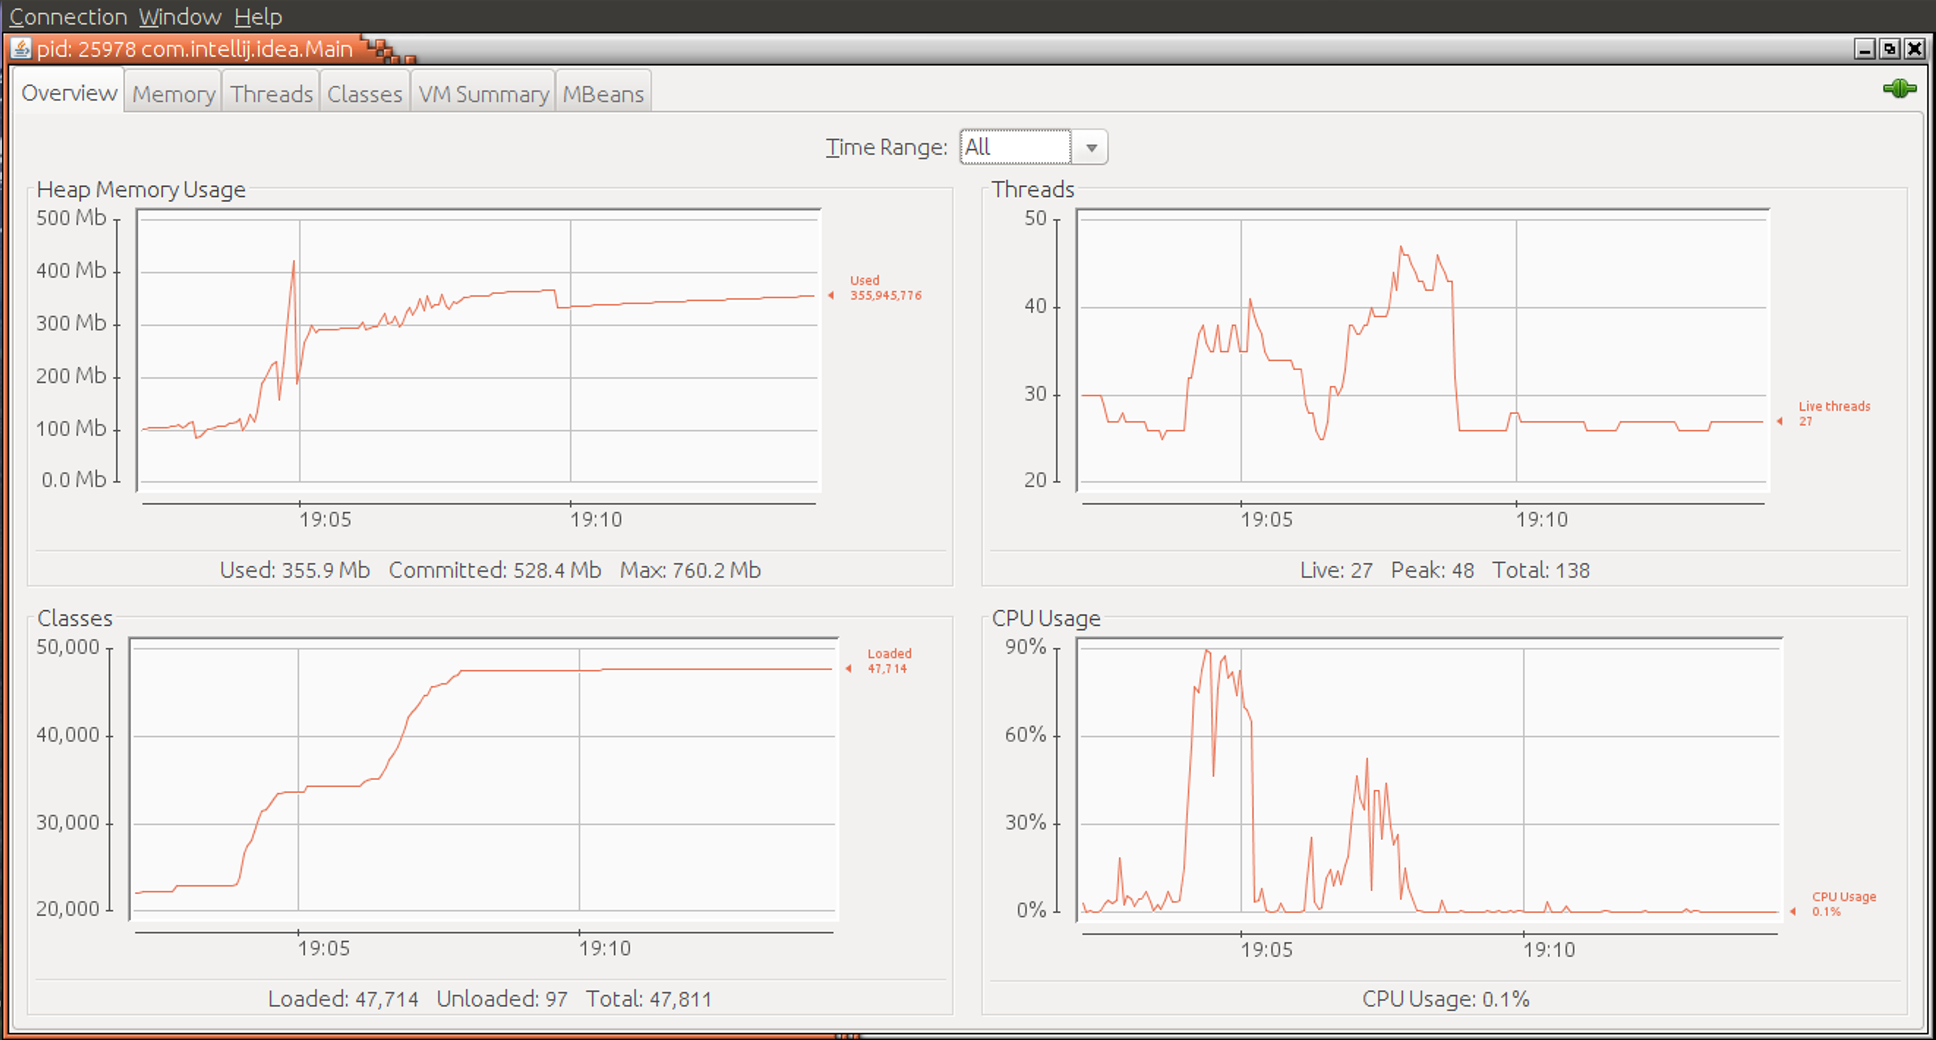
\includegraphics[width=13cm]{fig/jconsole.png}
	\caption{A JDK 8 JConsole tool main window. It shows use of resources, another tabs contain more detailed information and a facility to manage object called a MBeans.}
	\label{jconsole}
\end{figure}

\subsection{GC Viewer}
GC Viewer is a tool for analysis GC logs. Firstly, you have to run a JVM with options \texttt{-Xloggc:}\textit{logFile} \texttt{\seqsplit{-XX:+PrintGCDetails -XX:+PrintGCDateStamps}}, where \textit{logFile} is a file where GC events will be stored. Secondly, open the \textit{logFile} in the GC Viewer to assessment of effectiveness GC operations, memory footprint, heap usage, throughput and so on. Therefore GC Viewer is an offline tool.
This tool is completely written in Java language. Tagtraum industries\footnote{http://www.tagtraum.com/gcviewer.html} developed GC Viewer till 2008. Since this time it's open source project\footnote{Official repository is accessible at \url{https://github.com/chewiebug/GCViewer}} under GNU Lesser General Public License.\cite{gcviewer} The GC Viewer is being updated. All support JVMs are in table \ref{gcviewersupportsjvms}.

\begin{figure}[h]
	\centering
	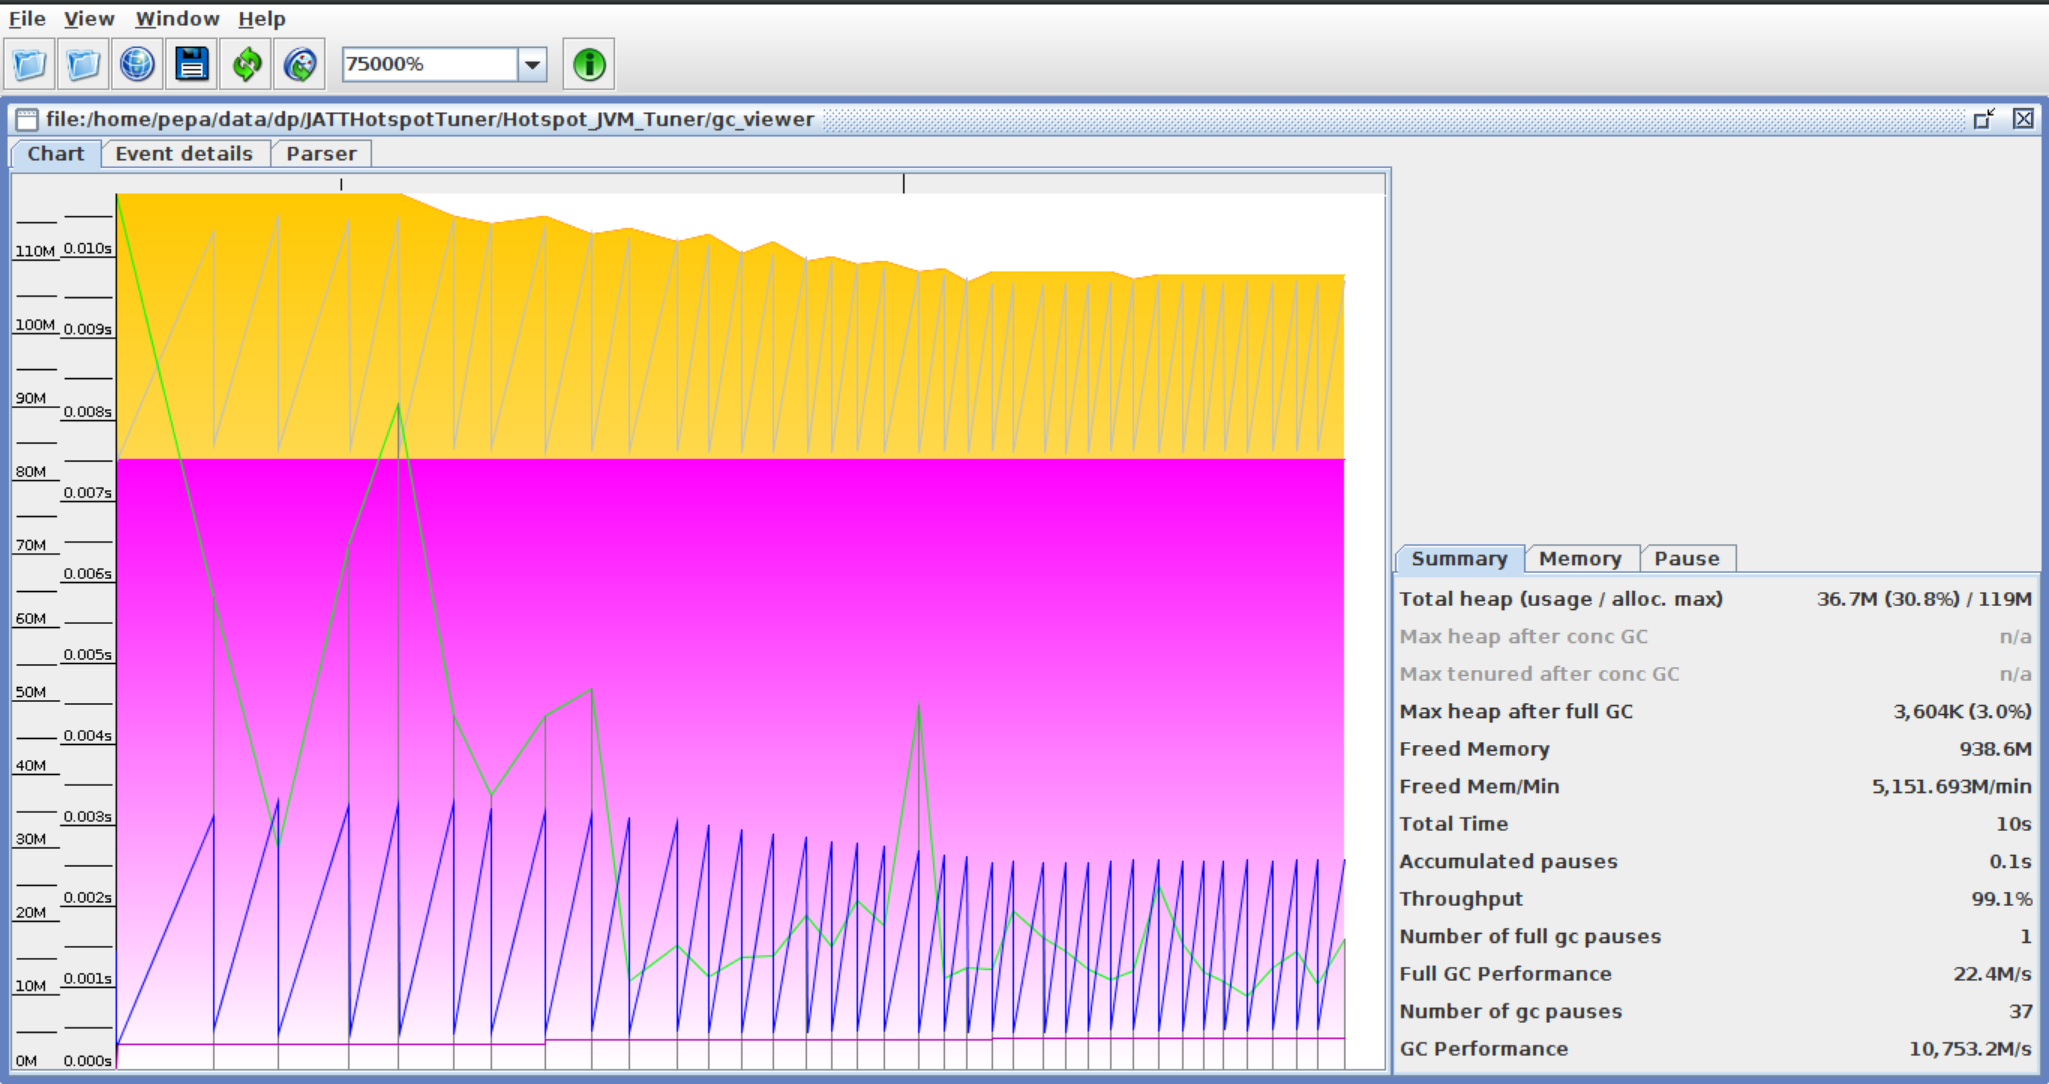
\includegraphics[width=13cm]{fig/gcviewer.png}
	\caption{A GC Viewer GUI. This tool is can be used to detailed analysis of GC logs.}
	\label{gcviwer}
\end{figure}


\section{Automatic optimization tools}\label{autoopt}

%TODO registruj se na https://www.dynatrace.com/trial/?vehicle_name=https://www.dynatrace.com/technologies/java-monitoring/ pro vyzkouseni dynatrace a pripadne s nim muzes pak neco zmerit a optimalizovat a zahrnout do prace.

\subsection{JATT}\label{jatt}
A JATT (JVM Auto Tuning Tool) is an open source software tool which was developed to optimize JVM. The JATT is based on the OpenTuner\footnote{"OpenTuner is a new framework for building domain-specific multi-objective program autotuners. OpenTuner supports fully customizable configuration representations, an extensible technique representation to allow for domain-specific techniques, and an easy to use interface for communicating with the tuned program." \url{http://opentuner.org/}} framework and it supports only the Linux environment. Aforementioned tool offers the Console mode and the Graphical User Interface as well. Authors highly recommend to use the console mode for more advanced work. The JATT is designed to tune especially HotSpot JVM (namely, it was tested on OpenJDK 7 update 55) but it can be modified to auto tune a different JVM.
\cite{jatt-web} \cite{jatt-web-dzone}
%TODO sel by trochu doplnit OpenTuner -- algoritmy, techniky hledani apod. podle http://groups.csail.mit.edu/commit/papers/2014/ansel-pact14-opentuner.pdf
%QT doplnit tuner
%QT Java 9, porovnat? Je modularni, coz by mohlo mit na performance. Koukni na https://docs.oracle.com/javase/9/whatsnew/toc.htm a tuning. Nektere options byly zakazany. G1 je defaultni GC,... Java 9 by take mela mit lepsi "self-tuning" (wikipedia).

The \textit{JATT} is an \textbf{offline} tuning tool -- it means a tuning phase and a production phase are strictly separated. Firstly, an optimal parameter configuration that will produce best performance within specified deployment environment. Secondly, found optimal configuration is used to deploy the application. There is an opposite approach called \textbf{online} tuning which deals with finding an optimal configuration during the runtime of an application. The \textit{JATT} does not offer an online auto tuning of JVM now but it is in development. 
% TODO napsat autorum, jestli je nastroj aktualne spravovany a jestli budou ve vyvoji pokracovat a podle toho dopsat
An initial phase of development indicates use of a \textit{jstat} utility\footnote{For more informations see sites \url{https://docs.oracle.com/javase/8/docs/technotes/guides/troubleshoot/tooldescr017.html} and \url{https://docs.oracle.com/javase/8/docs/technotes/tools/unix/jstat.html} for use.}. \cite{jatt}

Already stated tool is written in Python programming language\footnote{Official repository is located at \url{https://bitbucket.org/sapients/hotspottuner/}} and except for the OpenTuner it requires other packages. For a comprehensive information about requirements, installation and use see website \cite{jatt-web-medium}. There is shown a simple example of the Java application auto tuning and performance results are briefly discussed.

For logical division the JATT divides options into ten groups. We are able to auto tune JVM according to every group of our interest. Alongside this a searching space and a tuning time are reduced. We can easily use two or more groups at the same time or define own set of options to auto tune. All options are stored in \texttt{Flags} folder in \texttt{csv} files, including \texttt{Temporary} file which is predestined to input own list of options which the JATT will use to auto tune a JVM.

The JATT is student project which originated in 2012 at the University of Moratuwa, Sri Lanka. Project won the gold medal award at Association for Computing Machinery (ACM) student research competition attached to 2015 International Symposium on Code Generation and Optimization. \cite{jatt-web}

\begin{figure}[h]
	\centering
	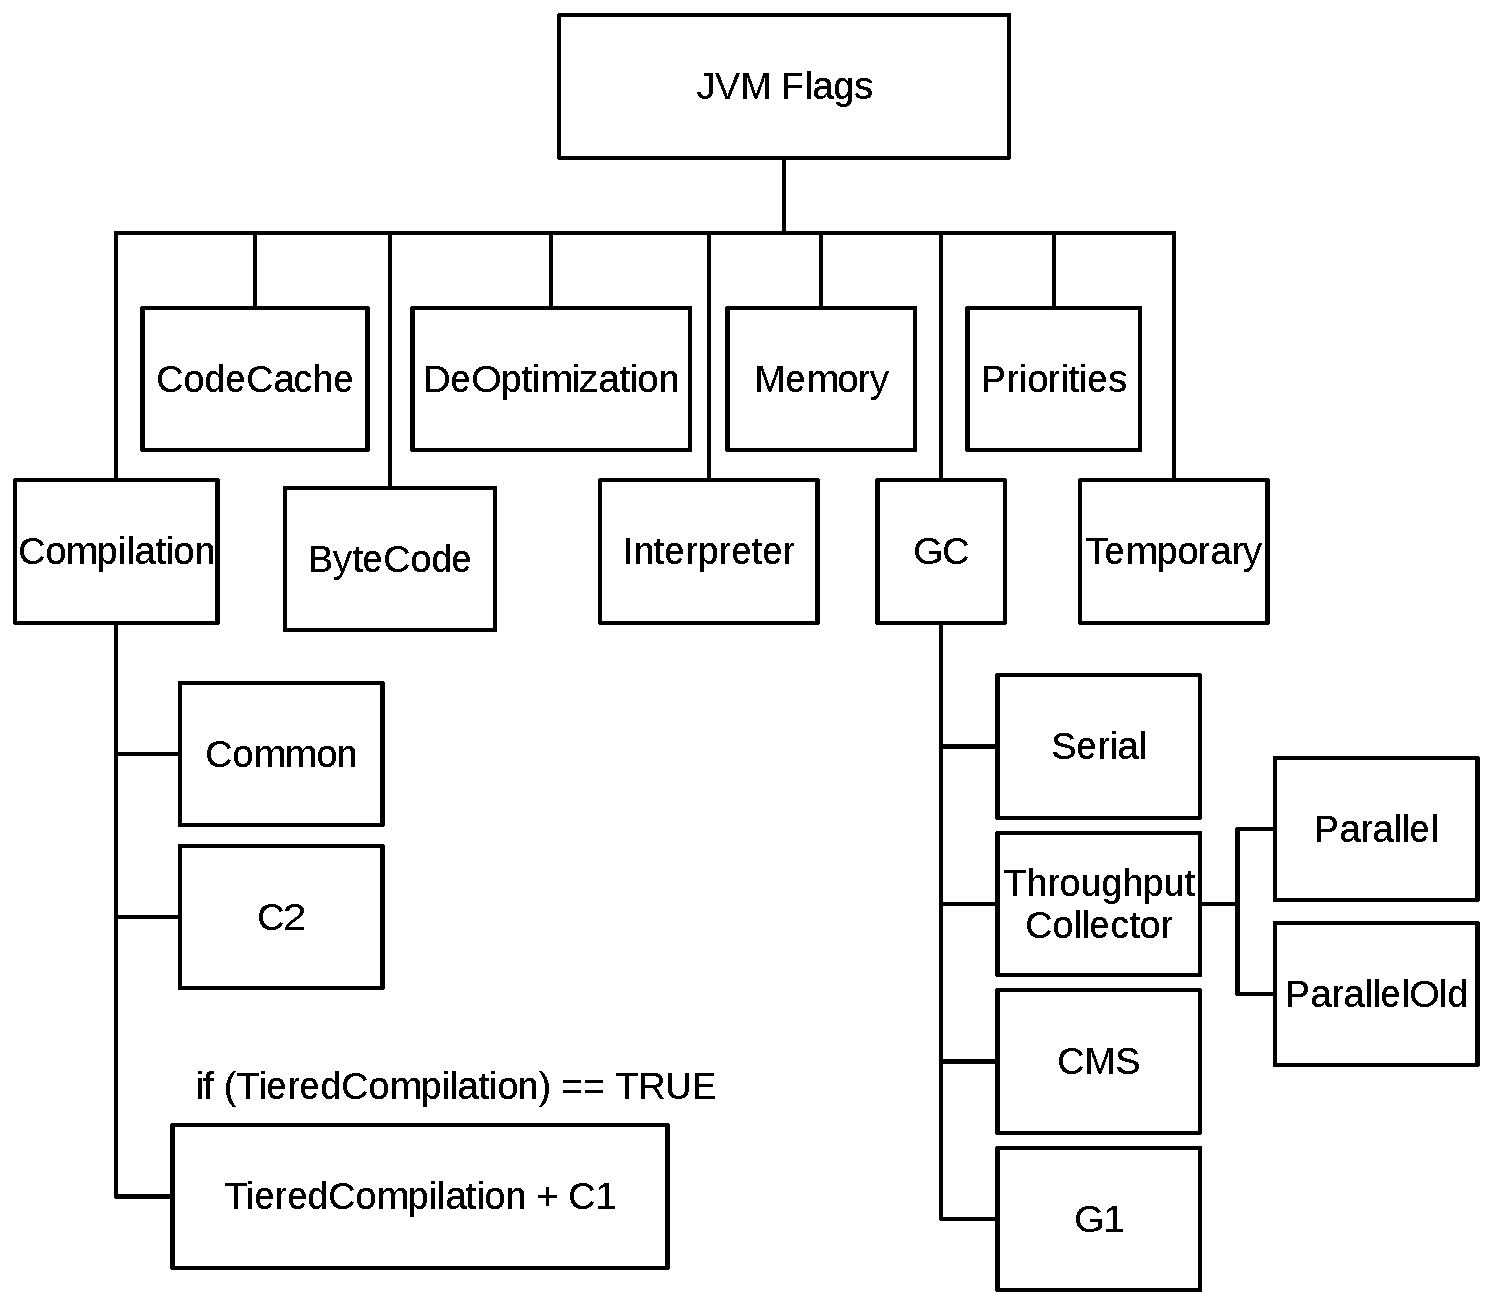
\includegraphics[width=13cm]{fig/flags.pdf}
	\caption{A JVM options hierarchy. The JATT divides JVM options into several groups. The division aims to reduce a searching space. But it's possible to use two or more groups together also. \cite{jatt-progress} \cite{jatt-web-medium}}
	\label{jatt-hierarchy}
\end{figure}

To start auto tuning Java application, find \texttt{JATTHotspotTuner} folder and type command in terminal: \newline \texttt{python src/javaProgramTuner.py -\--source=}\textit{application} \texttt{\seqsplit{\  -\--iterations=}}\textit{numberOfIterations} \texttt{\ -\--flags=}\textit{optionCategory} \texttt{\ -\--configfile=}\textit{\seqsplit{fileWithResults}} \newline

Parameters of command are:
\begin{itemize}
	\item \textit{application} -- Java application to auto tune (a \texttt{*.class} file)
	\item \textit{numberOfIterations} -- measured runtime is average of \textit{numberOfIterations} runs
	\item \textit{optionCategory} -- you can use one or more categories which are separated by commas (see picture \ref{jatt-hierarchy})
	\item \textit{fileWithResults} -- a text file will be stored in \texttt{\seqsplit{src/TunedConfiguration}} folder with found configurations. If you more times run command with same \textit{fileWithResults} data will not be overwritten while new records will be added. A result entry syntax is shown in figure \ref{jatt-result}
\end{itemize}

In figure \ref{jatt-result} is an example of \textit{fileWithResults} file. There is group(s) options configuration on the first line used to achieve given runtime. The \texttt{Improvement} represents ratio of improvements which is given by equation: $Improvement = Default\ metric / Runtime$ \cite{jatt-web-dzone}, where \texttt{Default metric} is the application runtime without changed JVM options. Result file ordinarily contains increasing entry sequence by improvement factor including a header with information about used option group(s) and tuning start time.
%TODO jvmtunerInterface.py je api ktere jde rozsirit, napr. javaProgramTuner.py, dacapoTuner.py, lze napsat i vlastni, pokud treba nebude aplikace mit jako vystup casovou jednotku, ktera je treba snizovat)
\begin{figure}[h]
	\flushleft{
	\texttt{\seqsplit{-XX:+Inline\ -XX:+ClipInlining\ -XX:+UseTypeProfile\ ...\ -XX:AutoBoxCacheMax=120\ -XX:EliminateAllocationArraySizeLimit=56\ -XX:ValueSearchLimit=1058\ ...}}
	\newline \texttt{Improvement: 1.05022358536}
	\newline \texttt{Runtime 0.114877080917}
	\newline \texttt{Default metric 0.120646619797}
	\newline \texttt{Configuration Found At: 2017-08-12 20:11:17.910694}}
	\caption{An example of the JATT result entry. An option configurations of group(s) (shorted here) and improvement factor are the most important information.}
	\label{jatt-result}
\end{figure}

%Co se tyce nastroju rad bych videl prehled / analyzu existujicich nastroju:
%- info jestli je nastroj udrzovan,
%- jestli je open source
%- licenci,
%- kdy vznikl,
%- cenu,
%- programovaci jazyk,
%- podporovany OS,
%- moznosti automatizace (API),
%- prehled zakladnich moznosti nastroju.
\subsection{ParamILS}
Philipp Lengauer and Hanspeter Mössenböck deal with automatic parameter tuning for Java Garbage Collectors \cite{jvmtuner}. They introduced a tool extensively based on ParamILS framework for JVM tuning, primarily for improving GC operations in 2014. The tool is practically short bash script which launch ParamILS with parameter model -- options for tuning divided by Garbage collector algorithms in ParamILS-specic syntax. Own tool is under the GNU General Public License and the ParamILS software is owned by Meta-Algorithmic Technologies Inc. and permission is hereby granted for non-commercial use\footnote{For commercial use contact Chris Fawcett, chris.fawcett@gmail.com}. \cite{jvmtuner} \cite{paramils} The ParamILS is a collection of easy readable Ruby scripts and both tools support Windows and Linux operating systems\footnote{\url{http://www.cs.ubc.ca/labs/beta/Projects/ParamILS/ParamILS-Quickstart.pdf}}. 


%TODO spoluprace s Dynatrace, popsat techniky jaho hill-climbing a dalsi, ktere ParamILS vyuziva
%TODO nezapomen porovnat tyto dva nastroje

\subsection{Commercial tools}
Among important non-freely accessible tools belong:
\begin{itemize}
	\item Arcturus Applicare\footnote{\url{http://www.arcturustech.com/tunewizard.html}} -- comprehensive tool for automated performance tuning, intelligent monitoring, optimization and instant root cause analysis. Applicable for great systems such web applications.
	\item Dynatrace -- this company is a leader for application performance monitoring and tuning for Java and .NET applications. Dynatrace collaborates with Philipp Lengauer and Hanspeter Mössenböck on JVM tuning. \cite{jvmtuner-boost}
	\item Plumbr\footnote{\url{https://plumbr.eu/}}
\end{itemize}




%{\color{red} In many cases, though, remember that the JVM is a small part of the overall performance picture. \cite{scott} p. 10}



% Dotazy
% Bezi cilova aplikace izolovane nebo jsou tam i dalsi java aplikace?

\chapter{Optimization JVM}

\section{Application}
%TODO zjistit jak je to s webovym serverem -- tzn. jestli by bylo mozny sehnat klienta, ktery bude na webovou aplikaci vysilat pozadavky a ladit tuto webovou aplikaci
%Throughput and footprint are best measured using metrics particular to the application. For example, the throughput of a web server may be tested using a client load generator, whereas the footprint of the server may be measured on the Solaris operating system using the pmap command. However, pauses due to garbage collection are easily estimated by inspecting the diagnostic output of the virtual machine itself.
%The command-line option -verbose:gc causes information about the heap and garbage collection to be printed at each collection. For example, here is output from a large server application:
%http://docs.oracle.com/javase/8/docs/technotes/guides/vm/gctuning/generations.html#sthref19
%strana 403 v \cite{hunt}

The DaCapo benchmark suite version 9.12 was chosen for the primal experimentation with JVM tuning. This suite includes these benchmarks: \cite{DaCapo:paper}
\begin{itemize}
	\item \textbf{antlr} -- A parser generator and translator generator
	\item \textbf{bloat} -- A bytecode-level optimization and analysis tool for Java
	\item \textbf{chart} -- A graph plotting toolkit and pdf renderer
	\item \textbf{eclipse} -- An integrated development environment (IDE)
	\item \textbf{fop} -- An output-independent print formatter
	\item \textbf{hsqldb} -- An SQL relational database engine written in Java
	\item \textbf{jython} -- A python interpreter written in Java
	\item \textbf{luindex} -- A text indexing tool
	\item \textbf{lusearch} -- A text search tool
	\item \textbf{pmd} -- A source code analyzer for Java
	\item \textbf{xalan} -- An XSLT processor for transforming XML documents
\end{itemize}
\section{Measurement methodology}
A machine with these parameters was used for measurement:
\begin{itemize}
	\item CPU -- Intel\textregistered\ Core\texttrademark\ i5-2450M, 2 cores, 4 threads
	\item Memory -- 8 GB
	\item Operating system -- Ubuntu 16.04, kernel Linux 4.10.0-33-generic (x86\_64)
\end{itemize}

Firstly, 10 runs of \textit{xalan} benchmark without warm-up period were realized. Measured values are in table \ref{default}. Secondly, an auto tuning tool was used to gain JVM options. Thirdly, 10 runs of \textit{xalan} benchmark with tuned options were realized again to observe performance changes.

%TODO dat tam taky mnou vybrane parametry z bigimpactu a provest mereni - temporary na xalanu
%TODO One particularly important case of testing a full application occurs when multiple applications are run at the same time on the same hardware. Many aspects of the JVM are	tuned by default to assume that all machine resources are available to them, and if those JVMs are tested in isolation, they will behave well. If they are tested when other applications are present (including, but not limited to, other JVMs), their performance will be quite different. \cite{scott} p. 18}

\section{JATT}
%TODO podle flagu to neni aktualni pro verzi Javy 8 -- ma tam jeste parametr MaxPermSize. Bude to potreba aktualizovat podle porovnani...
The JATT provides an interface to auto tune DaCapo benchmark. A command \texttt{\seqsplit{python\ src/dacapoTuner.py\ --source=xalan\ --iterations=1\ --flags=gc\ --configfile=dacapo\_results}} starts finding better JVM options settings with respect to GC operations. Searching took approximately an hour and result configuration is in figure \ref{jatttunedgcoptions}. \textit{Xalan} benchmark was performed with found JVM settings and measured values are in table \ref{jattgcresults}.

Average optimized runtime was 10415 milliseconds what in comparison to default value 11385 milliseconds is improvement by more than 8 \%. Accumulated GC pause is shorter more than four times. To the contrary, there is huge increase in memory footprint -- from original 128 MB to 742 MB. After detailed exploration logs in GC Viewer is apparent that only one GC event occurred.

A reduction runtime by 8 \% is significant together without any code adjustment. But memory consumption could be problematic, especially when a Java application runs on a machine with limited memory.

With the goal of reducing memory footprint another JATT flag was used -- namely \textit{memory} flag. Memory footprint has been reduced from original 128 MB to 37 MB with runtime improvement by 6 \%. In comparison to previous optimized JVM settings, there is runtime increase by approximately 2.5 \%.  Complete results are in table \ref{jattmemoryresults} and found options are in figure \ref{jatttunedmemoryoptions}.

In this part of thesis will be \textit{Big Impact} options (in table \ref{bigimpactprimitive}) tune. As was described in section \ref{jatt}, the JATT tool allows tuning own set of JVM options. Chosen options are stored in \texttt{\seqsplit{src/Flags/Temporary/temporary.csv}} file and auto tuning initiates same command but with \textit{temporary} flag. This file was filled with \textit{Big Impact Primitive} options.

The best options setting what JATT has found is in figure \ref{jatttunedbigimpactoptions}. \textit{Xalan} benchmark achieved average values 12009 milliseconds for runtime and 46 MB for memory footprint. It means the application has run by 5 \% longer than the application running in the JVM with the default settings and used about 82 MB less memory space. Measured values are in table \ref{jattbigimpactresults}.

Finally, auto tuning by JATT with all option set was initiated. The best JVM settings was found approximately in two hours. Overall searching phase took four hours but JATT could not improve settings  in the second half of auto tuning. Thanks to the using of all options runtime has been reduced by more than 20 \% at the expense of increment memory footprint from original 128 MB to 231 MB. Complete results are in the table \ref{jattalloptionsresults}.

%TODO
{\color{red} Vysledne nastaveni tedy obsahuje pres 600 parametru, coz se do papirove prilohy uz nevyda. Lze je prilozit jako elektronickou prilohu do archivu prace.}

\section{ParamILS}
This framework was used to optimize parameters stored in \texttt{\seqsplit{gc\_parameter\_model/params\_gc}} file which led to improvement time and space complexity as well. Specifically, \textit{Xalan} benchmark needed by 7 \% runtime and almost 60 \% memory space less to finish the test. Measured values are in the table \ref{ilsgcresults} and gained settings is in figure \ref{ilsgcoptions}.

\section{Comparison}
All results are enclosed in chapter \ref{results}. In next two figures are graphically compared measured data. Apparently, setting which leads to the fastest application run is simultaneously the most memory consumption. Settings gained by JATT with \textit{memory} flag and ParamILS with GC parameter model are better in both observed metrics.

When chosen \textit{Big Impact} options was used to tune a JVM setting, it led to deterioration of runtime and memory footprint as well. It could be caused by overly restricted option set and/or incorrect combination of options which JATT cannot improve.

\begin{figure}[h]
	\centering
	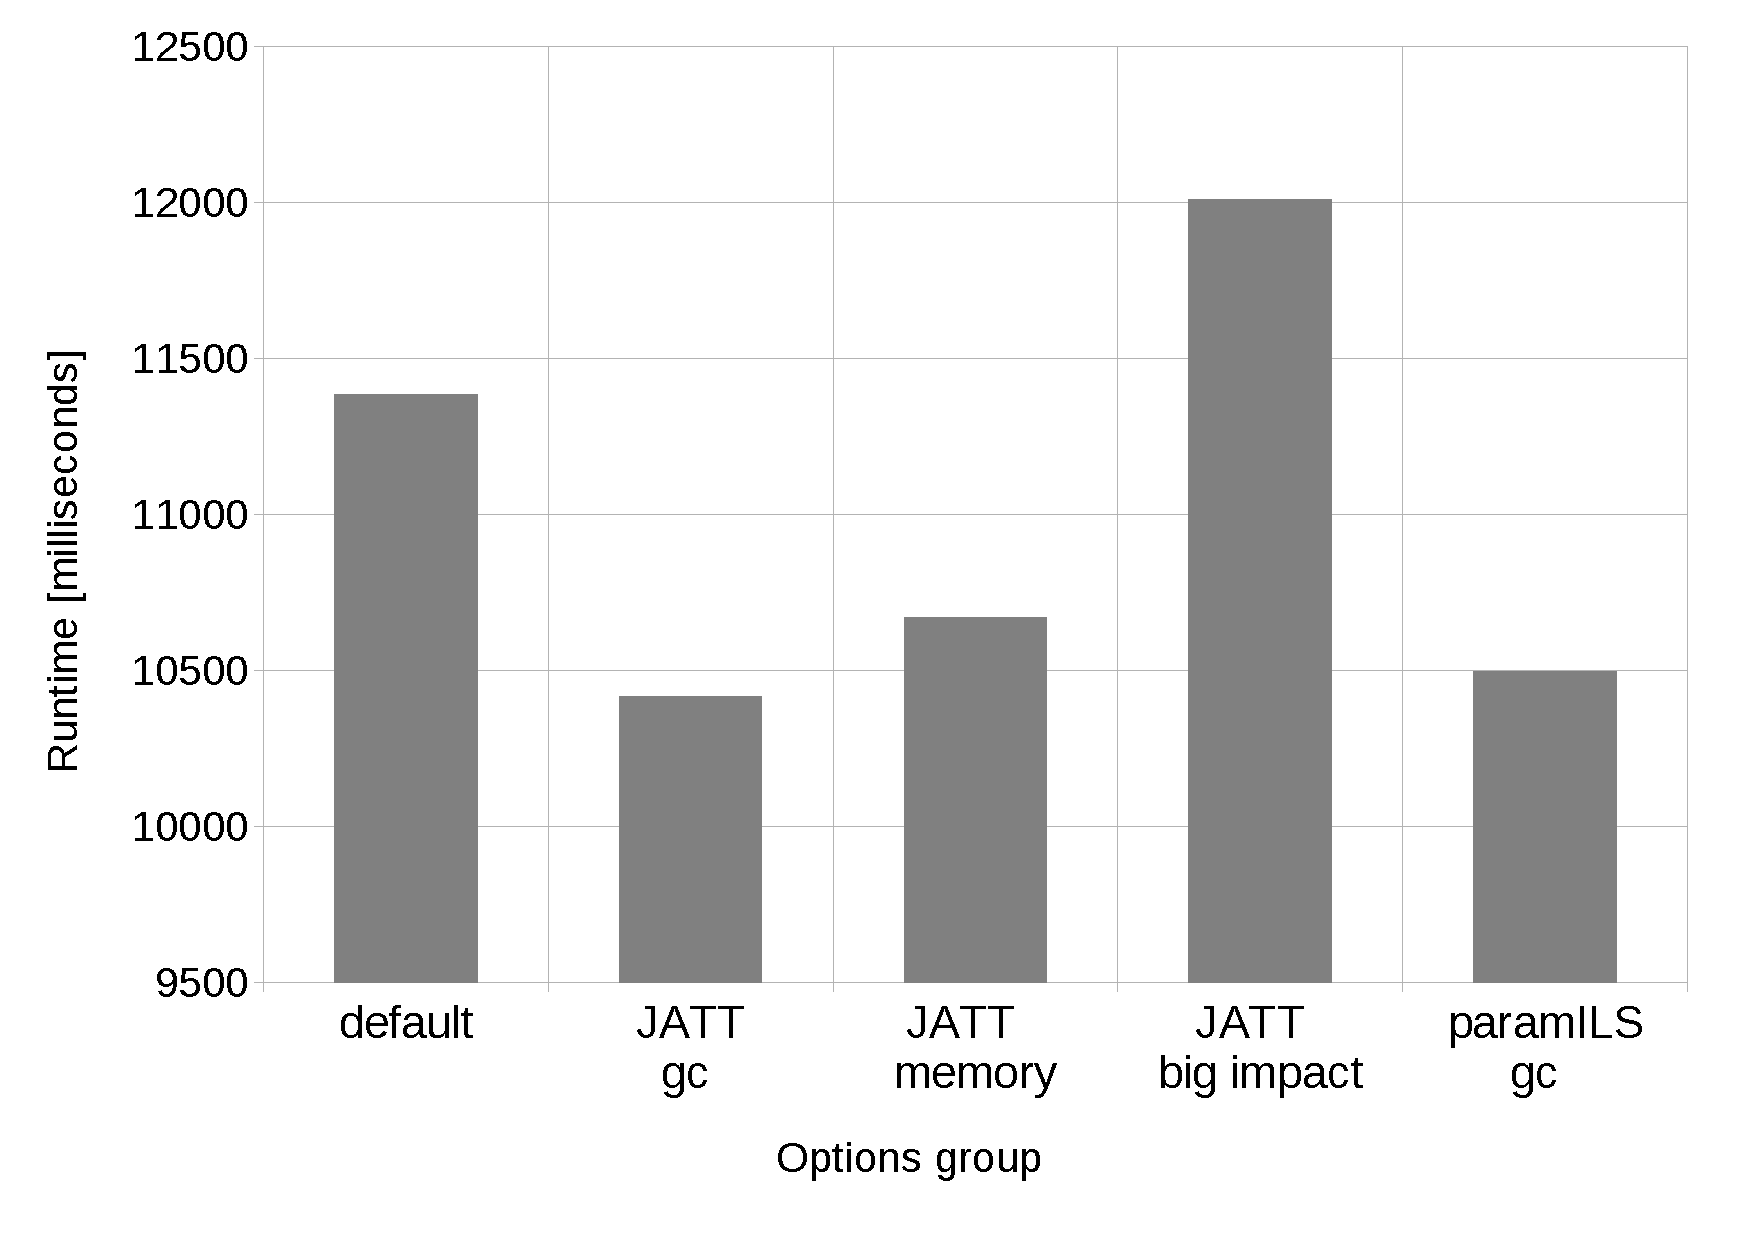
\includegraphics[width=13cm]{fig/runtimeBiggerFont.pdf}
	\caption{A comparison of an application runtime. Less is better.}
	\label{runtime}
\end{figure}

\begin{figure}[h]
	\centering
	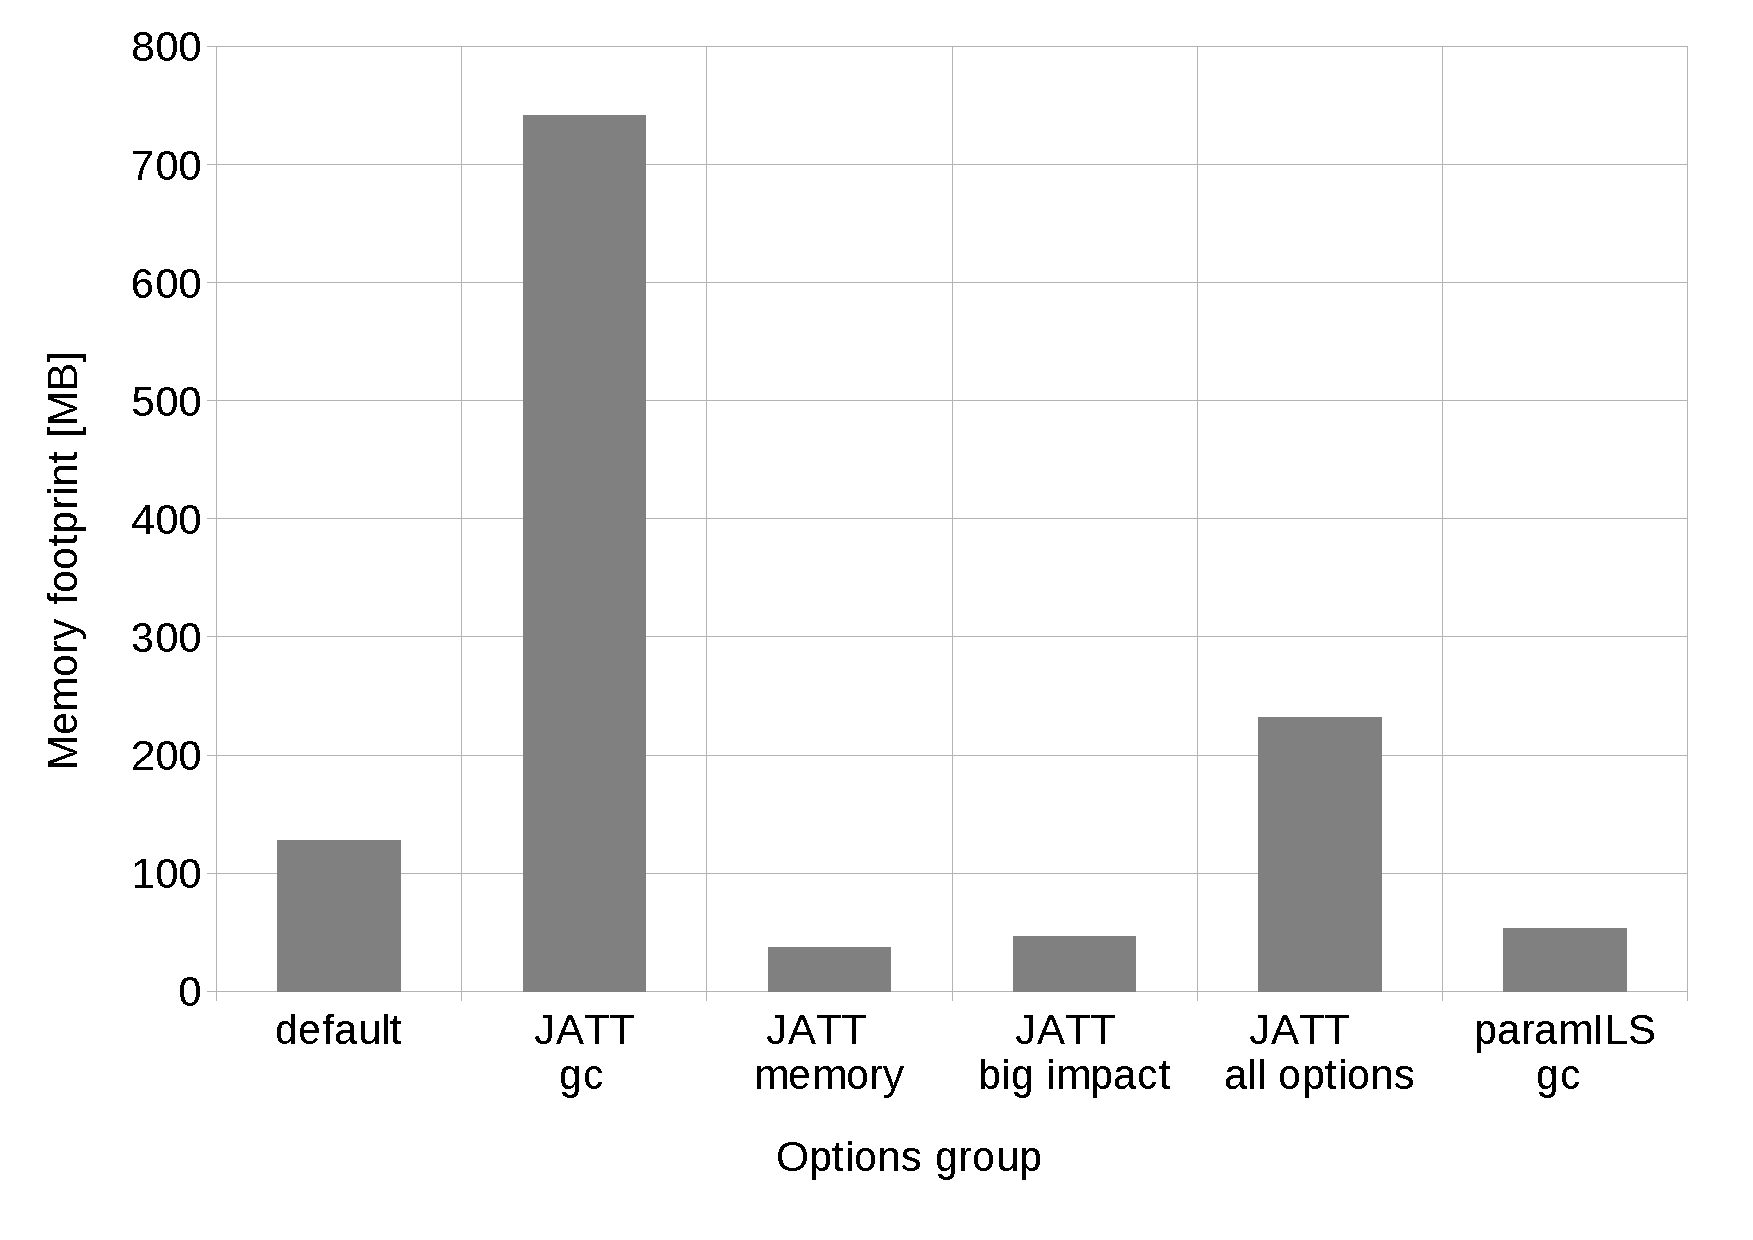
\includegraphics[width=13cm]{fig/footprintBiggerFont.pdf}
	\caption{An overall application memory footprint. Less is better.}
	\label{footprint}
\end{figure}

\clearpage
\chapter{Conclusion}
Will be written in the end.

\clearpage
\bibliographystyle{ieeetran}
\bibliography{bibfile}

\appendix
\chapter{Big impact options}
\begin{table}[]
	\centering
	\begin{tabular}{|l|l|}
		\hline
		-d32 | -d64                   & -XX:Inline                  \\ \hline
		-server | -client             & -XX:MaxGCPauseMillis        \\ \hline
		-Xmixed                       & -XX:MaxMetaspaceSize        \\ \hline
		-Xcomp                        & -XX:MaxNewSize              \\ \hline
		-Xint                         & -XX:MaxTenuringThreshold    \\ \hline
		-Xms						  & -XX:MetaspaceSize           \\ \hline
		-Xmx						  & -XX:NewRatio                \\ \hline
		-Xss						  & -XX:NewSize                 \\ \hline
		-XX:BackgroundCompilation     & -XX:SoftRefLRUPolicyMSPerMB \\ \hline
		-XX:CICompilerCount           & -XX:SurvivorRatio           \\ \hline
		-XX:CICompilerCountPerCPU     & -XX:ThreadStackSize         \\ \hline
		-XX:CompileThreshold          & -XX:UseBiasedLocking        \\ \hline
		-XX:DoEscapeAnalysis          & -XX:UseGCOverheadLimit      \\ \hline
		-XX:ErgoHeapSizeLimit         & -XX:UseParallelOldGC        \\ \hline
		-XX:InitialTenuringThreshold  & -XX:UseSerialGC             \\ \hline
	\end{tabular}
	\caption{The big impact primitive options. It's possible to use any option without enabling the other one. These options subject subsequent optimization.}
	\label{bigimpactprimitive}
\end{table}
	
	
	

\begin{table}[]
	\centering
	\begin{tabular}{|l|l|}
		\hline
		\multicolumn{2}{|l|}{\textbf{Complex}}                                              \\ \hline
		-server                                    & -XX:TieredCompilation                  \\ \hline
		\multirow{4}{*}{-XX:UseParallelGC}         & -XX:InitialSurvivorRatio               \\ \cline{2-2} 
		& -XX:MinSurvivorRatio                   \\ \cline{2-2} 
		& -XX:TargetSurvivorRatio                \\ \cline{2-2} 
		& -XX:GCTimeRatio                        \\ \hline
		\multirow{4}{*}{-XX:UseConcMarkSweepGC}    & -XX:CMSInitiatingOccupancyFraction     \\ \cline{2-2} 
		& -XX:UseCMSInitiatingOccupancyOnly      \\ \cline{2-2} 
		& -XX:ConcGCThreads                      \\ \cline{2-2} 
		& -XX:CMSClassUnloadingEnabled           \\ \hline
		\multirow{2}{*}{-XX:UseAdaptiveSizePolicy} & -XX:UseAdaptiveSizePolicyFootprintGoal \\ \cline{2-2} 
		& -XX:UseAdaptiveSizePolicyWithSystemGC  \\ \hline
		\multirow{3}{*}{-XX:UseG1GC}               & -XX:ConcGCThreads                      \\ \cline{2-2} 
		& -XX:UseStringDeduplication             \\ \cline{2-2} 
		& -XX:G1MixedGCLiveThresholdPercent      \\ \hline
		All GC except Serial GC                    & -XX:ParallelGCThreads                  \\ \hline
	\end{tabular}
	\caption{The big impact complex options. To use the option from the right column it's necessary to enable the  option from the left column. These options subject subsequent optimization.}
	\label{bigimpactcomplex}
\end{table}		

\begin{table}[]
	\centering
	\begin{tabular}{|l|}
		\hline
		preliminary support for OpenJDK 9 Shenandoah algorithm in unified \\ logging format \texttt{-Xlog:gc: -XX:+UseShenandoahGC  }   \\ \hline
		Oracle JDK 1.8 \texttt{-Xloggc: {[}-XX:+PrintGCDetails{]} {[}-XX:+PrintGCDateStamps{]}}                                      \\ \hline
		Sun / Oracle JDK 1.7 with option\\ \texttt{-Xloggc:} \texttt{{[}-XX:+PrintGCDetails{]} {[}-XX:+PrintGCDateStamps{]}}                    \\ \hline
		Sun / Oracle JDK 1.6 with option\\ \texttt{-Xloggc:} \texttt{{[}-XX:+PrintGCDetails{]} {[}-XX:+PrintGCDateStamps{]}}                    \\ \hline
		Sun JDK 1.4/1.5 with the option \texttt{-Xloggc: {[}-XX:+PrintGCDetails{]}}                                                  \\ \hline
		Sun JDK 1.2.2/1.3.1/1.4 with the option \texttt{-verbose:gc}                                                                 \\ \hline
		IBM JDK 1.3.1/1.3.0/1.2.2 with the option \texttt{-verbose:gc}                                                               \\ \hline
		IBM iSeries Classic JVM 1.4.2 with option \texttt{-verbose:gc}                                                               \\ \hline
		HP-UX JDK 1.2/1.3/1.4.x with the option \texttt{-Xverbosegc}                                                                 \\ \hline
		BEA JRockit 1.4.2/1.5/1.6 with the option \\\texttt{-verbose:memory {[}-Xverbose:gcpause,gcreport{]} {[}-Xverbosetimestamp{]}} \\ \hline
	\end{tabular}
	\caption{GC Viewer supports JVMs list. \url{https://github.com/chewiebug/GCViewer}}
	\label{gcviewersupportsjvms}
\end{table}

\chapter{Results}\label{results}
\begin{table}[]
	\centering
\begin{tabular}{|c|c|c|c|c|c|}
	\hline
	Run              & \begin{tabular}[c]{@{}c@{}}Runtime\\ {[}msec{]}\end{tabular} & \begin{tabular}[c]{@{}c@{}}Memory\\ Footprint \\ {[}MB{]}\end{tabular} & \begin{tabular}[c]{@{}c@{}}Accumul.\\ Pauses \\ {[}sec{]}\end{tabular} & \begin{tabular}[c]{@{}c@{}}Full GC\\ Perf.\\ {[}MB/s{]}\end{tabular} & \begin{tabular}[c]{@{}c@{}}GC\\ Perf.\\ {[}MB/s{]}\end{tabular} \\ \hline
	1                & 10716                                                        & 119                                                                    & 0.08                                                                   & 28.3                                                                 & 13937.1                                                         \\ \hline
	2                & 11100                                                        & 119                                                                    & 0.1                                                                    & 15.2                                                                 & 11384.2                                                         \\ \hline
	3                & 11882                                                        & 135                                                                    & 0.1                                                                    & 16.4                                                                 & 10167.9                                                         \\ \hline
	4                & 11268                                                        & 119                                                                    & 0.09                                                                   & 24.3                                                                 & 12406.4                                                         \\ \hline
	5                & 11513                                                        & 119                                                                    & 0.11                                                                   & 23.3                                                                 & 8924.2                                                          \\ \hline
	6                & 11539                                                        & 162.5                                                                  & 0.09                                                                   & 15.3                                                                 & 11932.2                                                         \\ \hline
	7                & 11163                                                        & 119                                                                    & 0.09                                                                   & 23.5                                                                 & 11662.3                                                         \\ \hline
	8                & 12043                                                        & 120                                                                    & 0.12                                                                   & 21.8                                                                 & 8300.6                                                          \\ \hline
	9                & 11325                                                        & 119                                                                    & 0.08                                                                   & 24                                                                   & 12755                                                           \\ \hline
	10               & 11300                                                        & 147                                                                    & 0.08                                                                   & 12.9                                                                 & 13569.9                                                         \\ \hline
	\textbf{Average} & \textbf{11385}                                               & \textbf{127.85}                                                        & \textbf{0.094}                                                         & \textbf{20.5}                                                        & \textbf{11503.98}                                               \\ \hline
\end{tabular}
	\caption{\textit{Xalan} benchmark runs in the default settings of the JVM.}
	\label{default}
\end{table}

\begin{table}[]
	\centering
	\begin{tabular}{|c|c|c|c|c|c|}
		\hline
		Run              & \begin{tabular}[c]{@{}c@{}}Runtime\\ {[}msec{]}\end{tabular} & \begin{tabular}[c]{@{}c@{}}Memory\\ Footprint \\ {[}MB{]}\end{tabular} & \begin{tabular}[c]{@{}c@{}}Accumul.\\ Pauses \\ {[}sec{]}\end{tabular} & \begin{tabular}[c]{@{}c@{}}Full GC\\ Perf.\\ {[}MB/s{]}\end{tabular} & \begin{tabular}[c]{@{}c@{}}GC\\ Perf.\\ {[}MB/s{]}\end{tabular} \\ \hline
		1                & 10397                                                        & 741.8                                                                  & 0.02                                                                   & 7857.2                                                               & 130215.7                                                        \\ \hline
		2                & 10633                                                        & 741.8                                                                  & 0.02                                                                   & 5357.2                                                               & 135230.5                                                        \\ \hline
		3                & 10249                                                        & 741.8                                                                  & 0.02                                                                   & 7933.9                                                               & 141060.9                                                        \\ \hline
		4                & 10521                                                        & 741.8                                                                  & 0.02                                                                   & 6213                                                                 & 120291.4                                                        \\ \hline
		5                & 10212                                                        & 741.8                                                                  & 0.02                                                                   & 6718.6                                                               & 88053.9                                                         \\ \hline
		6                & 10448                                                        & 741.8                                                                  & 0.02                                                                   & 5970.8                                                               & 97636.3                                                         \\ \hline
		7                & 10421                                                        & 741.8                                                                  & 0.02                                                                   & 7614.7                                                               & 131317.1                                                        \\ \hline
		8                & 10385                                                        & 741.8                                                                  & 0.02                                                                   & 6431.9                                                               & 98775.7                                                         \\ \hline
		9                & 10385                                                        & 741.8                                                                  & 0.03                                                                   & 8095.7                                                               & 39761.2                                                         \\ \hline
		10               & 10497                                                        & 741.8                                                                  & 0.02                                                                   & 5864.4                                                               & 109633.8                                                        \\ \hline
		\textbf{Average} & \textbf{10415}                                               & \textbf{741.8}                                                         & \textbf{0.021}                                                         & \textbf{6805.74}                                                     & \textbf{109197.65}                                              \\ \hline
	\end{tabular}
	\caption{\textit{Xalan} benchmark runs with settings found by JATT with \textit{gc} flag. Used settings is in a figure \ref{jatttunedgcoptions}}
	\label{jattgcresults}
\end{table}

\begin{table}[]
	\centering
	\begin{tabular}{|c|c|c|c|c|c|}
		\hline
		Run              & \begin{tabular}[c]{@{}c@{}}Runtime\\ {[}msec{]}\end{tabular} & \begin{tabular}[c]{@{}c@{}}Memory\\ Footprint \\ {[}MB{]}\end{tabular} & \begin{tabular}[c]{@{}c@{}}Accumul.\\ Pauses \\ {[}sec{]}\end{tabular} & \begin{tabular}[c]{@{}c@{}}Full GC\\ Perf.\\ {[}MB/s{]}\end{tabular} & \begin{tabular}[c]{@{}c@{}}GC\\ Perf.\\ {[}MB/s{]}\end{tabular} \\ \hline
		1                & 11203                                                        & 36.7                                                                   & 0.09                                                                   & 16.7                                                                 & 12548                                                           \\ \hline
		2                & 10571                                                        & 36.6                                                                   & 0.09                                                                   & 17.8                                                                 & 12601.3                                                         \\ \hline
		3                & 10627                                                        & 36.8                                                                   & 0.09                                                                   & 12.6                                                                 & 13282.9                                                         \\ \hline
		4                & 10379                                                        & 36.7                                                                   & 0.09                                                                   & 13.2                                                                 & 12.682                                                          \\ \hline
		5                & 10602                                                        & 36.7                                                                   & 0.08                                                                   & 24.4                                                                 & 14580.6                                                         \\ \hline
		6                & 10559                                                        & 36.7                                                                   & 0.09                                                                   & 14.5                                                                 & 12622.3                                                         \\ \hline
		7                & 10718                                                        & 36.6                                                                   & 0.08                                                                   & 23.6                                                                 & 13130.1                                                         \\ \hline
		8                & 11026                                                        & 36.8                                                                   & 0.09                                                                   & 18.9                                                                 & 12101.7                                                         \\ \hline
		9                & 10494                                                        & 36.7                                                                   & 0.09                                                                   & 24.1                                                                 & 11375.6                                                         \\ \hline
		10               & 10525                                                        & 36.7                                                                   & 0.09                                                                   & 19.1                                                                 & 11919.8                                                         \\ \hline
		\textbf{Average} & \textbf{10670}                                               & \textbf{36.7}                                                          & \textbf{0.088}                                                         & \textbf{18.49}                                                       & \textbf{11417.4982}                                             \\ \hline
	\end{tabular}
	\caption{\textit{Xalan} benchmark runs with settings found by JATT with \textit{memory} flag. Used settings is in a figure \ref{jatttunedmemoryoptions}}
	\label{jattmemoryresults}
\end{table}

\begin{table}[]
	\centering
	\begin{tabular}{|c|c|c|c|c|c|}
		\hline
		Run              & \begin{tabular}[c]{@{}c@{}}Runtime\\ {[}msec{]}\end{tabular} & \begin{tabular}[c]{@{}c@{}}Memory\\ Footprint \\ {[}MB{]}\end{tabular} & \begin{tabular}[c]{@{}c@{}}Accumul.\\ Pauses \\ {[}sec{]}\end{tabular} & \begin{tabular}[c]{@{}c@{}}Full GC\\ Perf.\\ {[}MB/s{]}\end{tabular} & \begin{tabular}[c]{@{}c@{}}GC\\ Perf.\\ {[}MB/s{]}\end{tabular} \\ \hline
		1                & 11934                                                        & 46.1                                                                   & 0.08                                                                   & 22.1                                                                 & 13831.4                                                         \\ \hline
		2                & 12034                                                        & 45.9                                                                   & 0.06                                                                   & 27.6                                                                 & 19230.4                                                         \\ \hline
		3                & 11950                                                        & 45.8                                                                   & 0.06                                                                   & 22.3                                                                 & 18530                                                           \\ \hline
		4                & 12034                                                        & 46                                                                     & 0.07                                                                   & 23                                                                   & 16739.3                                                         \\ \hline
		5                & 12083                                                        & 46                                                                     & 0.07                                                                   & 37                                                                   & 14005.5                                                         \\ \hline
		6                & 11984                                                        & 46.1                                                                   & 0.07                                                                   & 30.8                                                                 & 15018.3                                                         \\ \hline
		7                & 12152                                                        & 46                                                                     & 0.06                                                                   & 26.8                                                                 & 18473.5                                                         \\ \hline
		8                & 12035                                                        & 46.1                                                                   & 0.07                                                                   & 24                                                                   & 16687.3                                                         \\ \hline
		9                & 12000                                                        & 46.1                                                                   & 0.06                                                                   & 33.3                                                                 & 19396.4                                                         \\ \hline
		10               & 11880                                                        & 46.1                                                                   & 0.06                                                                   & 25.1                                                                 & 17798                                                           \\ \hline
		\textbf{Average} & \textbf{12009}                                               & \textbf{46.02}                                                         & \textbf{0.066}                                                         & \textbf{27.2}                                                        & \textbf{16971.01}                                               \\ \hline
	\end{tabular}
	\caption{\textit{Xalan} benchmark runs with settings found by JATT with temporary -- big impact options. Used settings is in a figure \ref{jatttunedbigimpactoptions}}
	\label{jattbigimpactresults}
\end{table}

\begin{table}[]
	\centering
	\begin{tabular}{|c|c|c|c|c|c|}
		\hline
		Run              & \begin{tabular}[c]{@{}c@{}}Runtime\\ {[}msec{]}\end{tabular} & \begin{tabular}[c]{@{}c@{}}Memory\\ Footprint\\ {[}MB{]}\end{tabular} & \begin{tabular}[c]{@{}c@{}}Accumul.\\ Pauses\\ {[}sec{]}\end{tabular} & \begin{tabular}[c]{@{}c@{}}Full GC\\ Perf.\\ {[}MB/s{]}\end{tabular} & \begin{tabular}[c]{@{}c@{}}GC\\ Perf.\\ {[}MB/s{]}\end{tabular} \\ \hline
		1                & 8707                                                         & 231.3                                                                 & 0.03                                                                  & 879.9                                                                & 67354.3                                                         \\ \hline
		2                & 8949                                                         & 231.4                                                                 & 0.03                                                                  & 1523.2                                                               & 74420.9                                                         \\ \hline
		3                & 8794                                                         & 231.4                                                                 & 0.03                                                                  & 2100.2                                                               & 71483.6                                                         \\ \hline
		4                & 8731                                                         & 231.3                                                                 & 0.03                                                                  & 1600.6                                                               & 73481.3                                                         \\ \hline
		5                & 8750                                                         & 231.5                                                                 & 0.03                                                                  & 1874.4                                                               & 72028.1                                                         \\ \hline
		6                & 8740                                                         & 231.5                                                                 & 0.03                                                                  & 1590.3                                                               & 72196.1                                                         \\ \hline
		7                & 8734                                                         & 231.4                                                                 & 0.03                                                                  & 1557.1                                                               & 60351.8                                                         \\ \hline
		8                & 8742                                                         & 231.5                                                                 & 0.04                                                                  & 1049.7                                                               & 57957.4                                                         \\ \hline
		9                & 8736                                                         & 231.3                                                                 & 0.02                                                                  & 1962.3                                                               & 73589.8                                                         \\ \hline
		10               & 8791                                                         & 231.5                                                                 & 0.05                                                                  & 1986.8                                                               & 26118.7                                                         \\ \hline
		\textbf{Average} & \textbf{8767}                                                & \textbf{231.41}                                                       & \textbf{0.032}                                                        & \textbf{1612.45}                                                     & \textbf{64898.2}                                                \\ \hline
	\end{tabular}
	\caption{\textit{Xalan} benchmark runs with settings found by JATT for all options.}
	\label{jattalloptionsresults}
\end{table}

\begin{table}[]
	\centering
	\begin{tabular}{|c|c|c|c|c|c|}
		\hline
		Run              & \begin{tabular}[c]{@{}c@{}}Runtime\\ {[}msec{]}\end{tabular} & \begin{tabular}[c]{@{}c@{}}Memory\\ Footprint \\ {[}MB{]}\end{tabular} & \begin{tabular}[c]{@{}c@{}}Accumul.\\ Pauses \\ {[}sec{]}\end{tabular} & \begin{tabular}[c]{@{}c@{}}Full GC\\ Perf.\\ {[}MB/s{]}\end{tabular} & \begin{tabular}[c]{@{}c@{}}GC\\ Perf.\\ {[}MB/s{]}\end{tabular} \\ \hline
		1                & 10562                                                        & 52.7                                                                   & 0.07                                                                   & n/a                                                                  & 13680.5                                                         \\ \hline
		2                & 10595                                                        & 52.9                                                                   & 0.06                                                                   & n/a                                                                  & 16334.1                                                         \\ \hline
		3                & 10197                                                        & 52.7                                                                   & 0.06                                                                   & n/a                                                                  & 16309.2                                                         \\ \hline
		4                & 10202                                                        & 52.9                                                                   & 0.06                                                                   & n/a                                                                  & 16146.6                                                         \\ \hline
		5                & 10663                                                        & 52.7                                                                   & 0.07                                                                   & n/a                                                                  & 14377.5                                                         \\ \hline
		6                & 10660                                                        & 52.9                                                                   & 0.07                                                                   & n/a                                                                  & 13791.2                                                         \\ \hline
		7                & 10430                                                        & 52.9                                                                   & 0.08                                                                   & n/a                                                                  & 12153.7                                                         \\ \hline
		8                & 10683                                                        & 52.9                                                                   & 0.07                                                                   & n/a                                                                  & 12806.3                                                         \\ \hline
		9                & 10457                                                        & 53                                                                     & 0.06                                                                   & n/a                                                                  & 16134.5                                                         \\ \hline
		10               & 10523                                                        & 52.9                                                                   & 0.06                                                                   & n/a                                                                  & 15632.7                                                         \\ \hline
		\textbf{Average} & \textbf{10497}                                               & \textbf{52.85}                                                         & \textbf{0.066}                                                         & \textbf{n/a}                                                         & \textbf{14736.63}                                               \\ \hline
	\end{tabular}
	\caption{\textit{Xalan} benchmark runs with settings found by ParamILS with GC parameters model. Used settings is in a figure \ref{ilsgcoptions}}
	\label{ilsgcresults}
\end{table}

\begin{figure}[h]
	\texttt{\seqsplit{-XX:+UseParNewGC\ -XX:+ParGCUseLocalOverflow\ -XX:-ParGCTrimOverflow\ -XX:-CMSParallelRemarkEnabled\ -XX:-CMSParallelSurvivorRemarkEnabled\ -XX:-CMSPLABRecordAlways\ -XX:+CMSConcurrentMTEnabled\ -XX:ParGCArrayScanChunk=66\ -XX:ParGCDesiredObjsFromOverflowList=25\ -XX:CMSYoungGenPerWorker=83001713\ -XX:-UseConcMarkSweepGC\ -XX:+ResizePLAB\ -XX:+ResizeOldPLAB\ -XX:+AlwaysPreTouch\ -XX:+ParallelRefProcEnabled\ -XX:+ParallelRefProcBalancingEnabled\ -XX:+UseTLAB\ -XX:+ResizeTLAB\ -XX:-ZeroTLAB\ -XX:-FastTLABRefill\ -XX:+NeverActAsServerClassMachine\ -XX:+AlwaysActAsServerClassMachine\ -XX:-UseAutoGCSelectPolicy\ -XX:-UseAdaptiveSizePolicy\ -XX:-UsePSAdaptiveSurvivorSizePolicy\ -XX:-UseAdaptiveGenerationSizePolicyAtMinorCollection\ -XX:+UseAdaptiveGenerationSizePolicyAtMajorCollection\ -XX:+UseAdaptiveSizePolicyWithSystemGC\ -XX:-UseAdaptiveGCBoundary\ -XX:-UseAdaptiveSizePolicyFootprintGoal\ -XX:-UseAdaptiveSizeDecayMajorGCCost\ -XX:+UseGCOverheadLimit\ -XX:-DisableExplicitGC\ -XX:+CollectGen0First\ -XX:-BindGCTaskThreadsToCPUs\ -XX:-UseGCTaskAffinity\ -XX:YoungPLABSize=5237\ -XX:OldPLABSize=836\ -XX:GCTaskTimeStampEntries=263\ -XX:TargetPLABWastePct=10\ -XX:PLABWeight=37\ -XX:OldPLABWeight=50\ -XX:MarkStackSize=4875124\ -XX:MarkStackSizeMax=370523639\ -XX:RefDiscoveryPolicy=0\ -XX:InitiatingHeapOccupancyPercent=27\ -XX:MaxRAM=200187289457\ -XX:ErgoHeapSizeLimit=0\ -XX:MaxRAMFraction=2\ -XX:DefaultMaxRAMFraction=6\ -XX:MinRAMFraction=3\ -XX:InitialRAMFraction=69\ -XX:AutoGCSelectPauseMillis=7432\ -XX:AdaptiveSizeThroughPutPolicy=0\ -XX:AdaptiveSizePausePolicy=0\ -XX:AdaptiveSizePolicyInitializingSteps=18\ -XX:AdaptiveSizePolicyOutputInterval=0\ -XX:AdaptiveSizePolicyWeight=15\ -XX:AdaptiveTimeWeight=25\ -XX:PausePadding=0\ -XX:PromotedPadding=3\ -XX:SurvivorPadding=1\ -XX:ThresholdTolerance=10\ -XX:AdaptiveSizePolicyCollectionCostMargin=30\ -XX:YoungGenerationSizeIncrement=28\ -XX:YoungGenerationSizeSupplement=79\ -XX:YoungGenerationSizeSupplementDecay=6\ -XX:TenuredGenerationSizeIncrement=28\ -XX:TenuredGenerationSizeSupplement=43\ -XX:TenuredGenerationSizeSupplementDecay=3\ -XX:MaxGCPauseMillis=16793486230599948288\ -XX:GCPauseIntervalMillis=0\ -XX:MaxGCMinorPauseMillis=12369914655517609984\ -XX:GCTimeRatio=145\ -XX:AdaptiveSizeDecrementScaleFactor=4\ -XX:AdaptiveSizeMajorGCDecayTimeScale=14\ -XX:MinSurvivorRatio=2\ -XX:InitialSurvivorRatio=4\ -XX:BaseFootPrintEstimate=391267844\ -XX:GCHeapFreeLimit=3\ -XX:PrefetchCopyIntervalInBytes=766\ -XX:PrefetchScanIntervalInBytes=534\ -XX:PrefetchFieldsAhead=1\ -XX:ProcessDistributionStride=5}}
	\label{jatttunedgcoptions}
	\caption{JVM options for \textit{xalan} benchmark found by JATT with \textit{gc} flag.}
\end{figure}



\begin{figure}[h]
	\texttt{\seqsplit{-XX:-UseSharedSpaces\ -XX:+RequireSharedSpaces\ -XX:-DumpSharedSpaces\ -XX:+RelaxAccessControlCheck\ -XX:+UseVMInterruptibleIO\ -XX:ThreadSafetyMargin=72943233\ -XX:StackYellowPages=2\ -XX:StackShadowPages=25\ -XX:ThreadStackSize=1328\ -XX:VMThreadStackSize=1304\ -XX:CompilerThreadStackSize=0\ -XX:SharedReadWriteSize=16288215\ -XX:SharedReadOnlySize=10350874\ -XX:SharedMiscDataSize=5788599\ -XX:SharedMiscCodeSize=77206}}
	\label{jatttunedmemoryoptions}
	\caption{JVM options for \textit{xalan} benchmark found by JATT with \textit{memory} flag.}
\end{figure}

\begin{figure}[h]
	\texttt{\seqsplit{-XX:+BackgroundCompilation\ -XX:+CICompilerCountPerCPU\ -XX:+DoEscapeAnalysis\ -XX:-Inline\ -XX:-UseBiasedLocking\ -XX:-UseGCOverheadLimit\ -XX:-UseParallelOldGC\ -XX:-UseSerialGC\ -XX:CICompilerCount=4\ -XX:CompileThreshold=7316\ -XX:ErgoHeapSizeLimit=0\ -XX:InitialTenuringThreshold=4\ -XX:MaxGCPauseMillis=20402228389095275883\ -XX:MaxMetaspaceSize=26274393909091921920\ -XX:MaxNewSize=718203203\ -XX:MaxTenuringThreshold=13\ -XX:MetaspaceSize=20627973\ -XX:NewRatio=2\ -XX:NewSize=47816779\ -XX:SoftRefLRUPolicyMSPerMB=1229\ -XX:SurvivorRatio=9\ -XX:ThreadStackSize=1399}}
	\label{jatttunedbigimpactoptions}
	\caption{JVM options for \textit{xalan} benchmark found by JATT with \textit{temporary -- big impact} options.}
\end{figure}

\begin{figure}[h]
	\texttt{\seqsplit{-XX:MaxHeapFreeRatio=90\ -XX:AdaptiveSizeMajorGCDecayTimeScale=15\ -XX:YoungGenerationSizeSupplement=90\ -XX:AdaptiveSizeThroughPutPolicy=1\ -XX:YoungGenerationSizeSupplementDecay=2\ -XX:-ResizePLAB\ -XX:+DisableExplicitGC\ -XX:TenuredGenerationSizeSupplement=70\ -XX:TenuredGenerationSizeSupplementDecay=16\ -XX:MinSurvivorRatio=2\ -XX:+BindGCTaskThreadsToCPUs\ -XX:MaxTenuringThreshold=4\ -XX:NewRatio=1\ -XX:-UseAdaptiveSizePolicy\ -XX:MinHeapFreeRatio=10\ -XX:YoungPLABSize=1024\ -XX:-UseAdaptiveSizeDecayMajorGCCost\ -XX:+CollectGen0First\ -XX:AdaptiveSizePausePolicy=1\ -XX:AdaptiveSizePolicyInitializingSteps=80\ -XX:PLABWeight=80\ -XX:YoungGenerationSizeIncrement=10\ -XX:AdaptiveSizePolicyWeight=40\ -XX:+UseAdaptiveSizePolicyWithSystemGC\ -XX:AdaptiveSizeDecrementScaleFactor=2}}
	\label{ilsgcoptions}
	\caption{JVM options for \textit{xalan} benchmark found by ParamILS with gc parameters model.}
\end{figure}


\end{document}
